\documentclass{report}

%%%%%%%%%%%%%%%%%%%%%%%%%%%%%%%%%
% PACKAGE IMPORTS
%%%%%%%%%%%%%%%%%%%%%%%%%%%%%%%%%
\usepackage[dvipsnames]{xcolor}




\usepackage{anyfontsize}


\usepackage[tmargin=2cm,rmargin=1in,lmargin=1in,margin=0.85in,bmargin=2cm,footskip=.2in]{geometry}
\usepackage{amsmath,amsfonts,amsthm,amssymb,mathtools}
%\usepackage[varbb]{newpxmath}
\usepackage{xfrac}
\usepackage[makeroom]{cancel}
\usepackage{mathtools}
\usepackage{bookmark}
\usepackage{enumitem}
\usepackage{hyperref,theoremref}
\hypersetup{
	pdftitle={Assignment},
	colorlinks=true, linkcolor=doc!90,
	bookmarksnumbered=true,
	bookmarksopen=true
}
\usepackage[most,many,breakable]{tcolorbox}
\usepackage{xcolor}
\usepackage{varwidth}
\usepackage{varwidth}
\usepackage{etoolbox}
%\usepackage{authblk}
\usepackage{nameref}
\usepackage{multicol,array}
\usepackage{tikz-cd}
\usepackage[ruled,vlined,linesnumbered]{algorithm2e}
\usepackage{comment} % enables the use of multi-line comments (\ifx \fi) 
\usepackage{import}
\usepackage{xifthen}
\usepackage{pdfpages}
\usepackage{transparent}

\usetikzlibrary{shapes.geometric}
\usetikzlibrary{shapes}

\usetikzlibrary{calc}

\newcommand\mycommfont[1]{\footnotesize\ttfamily\textcolor{blue}{#1}}
\SetCommentSty{mycommfont}
\newcommand{\incfig}[1]{%
    \def\svgwidth{\columnwidth}
    \import{./figures/}{#1.pdf_tex}
}

\usepackage{tikzsymbols}
\renewcommand\qedsymbol{\sus}


%\usepackage{import}
%\usepackage{xifthen}
%\usepackage{pdfpages}
%\usepackage{transparent}


%%%%%%%%%%%%%%%%%%%%%%%%%%%%%%
% SELF MADE COLORS
%%%%%%%%%%%%%%%%%%%%%%%%%%%%%%



\definecolor{myg}{RGB}{56, 140, 70}
\definecolor{myb}{RGB}{45, 111, 177}
\definecolor{myr}{RGB}{199, 68, 64}
\definecolor{mytheorembg}{HTML}{F2F2F9}
\definecolor{mytheoremfr}{HTML}{00007B}
\definecolor{mylenmabg}{HTML}{FFFAF8}
\definecolor{mylenmafr}{HTML}{983b0f}
\definecolor{mypropbg}{HTML}{f2fbfc}
\definecolor{mypropfr}{HTML}{191971}
\definecolor{myexamplebg}{HTML}{F2FBF8}
\definecolor{myexamplefr}{HTML}{88D6D1}
\definecolor{myexampleti}{HTML}{2A7F7F}
\definecolor{mydefinitbg}{HTML}{E5E5FF}
\definecolor{mydefinitfr}{HTML}{3F3FA3}
\definecolor{notesgreen}{RGB}{0,162,0}
\definecolor{myp}{RGB}{197, 92, 212}
\definecolor{mygr}{HTML}{2C3338}
\definecolor{myred}{RGB}{127,0,0}
\definecolor{myyellow}{RGB}{169,121,69}
\definecolor{myexercisebg}{HTML}{F2FBF8}
\definecolor{myexercisefg}{HTML}{88D6D1}


%%%%%%%%%%%%%%%%%%%%%%%%%%%%
% TCOLORBOX SETUPS
%%%%%%%%%%%%%%%%%%%%%%%%%%%%

\setlength{\parindent}{1cm}
%================================
% THEOREM BOX
%================================

\tcbuselibrary{theorems,skins,hooks}
\newtcbtheorem[number within=section]{Theorem}{Theorem}
{%
	enhanced,
	breakable,
	colback = mytheorembg,
	frame hidden,
	boxrule = 0sp,
	borderline west = {2pt}{0pt}{mytheoremfr},
	sharp corners,
	detach title,
	before upper = \tcbtitle\par\smallskip,
	coltitle = mytheoremfr,
	fonttitle = \bfseries\sffamily,
	description font = \mdseries,
	separator sign none,
	segmentation style={solid, mytheoremfr},
}
{th}

\tcbuselibrary{theorems,skins,hooks}
\newtcbtheorem[number within=chapter]{theorem}{Theorem}
{%
	enhanced,
	breakable,
	colback = mytheorembg,
	frame hidden,
	boxrule = 0sp,
	borderline west = {2pt}{0pt}{mytheoremfr},
	sharp corners,
	detach title,
	before upper = \tcbtitle\par\smallskip,
	coltitle = mytheoremfr,
	fonttitle = \bfseries\sffamily,
	description font = \mdseries,
	separator sign none,
	segmentation style={solid, mytheoremfr},
}
{th}


\tcbuselibrary{theorems,skins,hooks}
\newtcolorbox{Theoremcon}
{%
	enhanced
	,breakable
	,colback = mytheorembg
	,frame hidden
	,boxrule = 0sp
	,borderline west = {2pt}{0pt}{mytheoremfr}
	,sharp corners
	,description font = \mdseries
	,separator sign none
}

%================================
% Corollery
%================================
\tcbuselibrary{theorems,skins,hooks}
\newtcbtheorem[number within=section]{Corollary}{Corollary}
{%
	enhanced
	,breakable
	,colback = myp!10
	,frame hidden
	,boxrule = 0sp
	,borderline west = {2pt}{0pt}{myp!85!black}
	,sharp corners
	,detach title
	,before upper = \tcbtitle\par\smallskip
	,coltitle = myp!85!black
	,fonttitle = \bfseries\sffamily
	,description font = \mdseries
	,separator sign none
	,segmentation style={solid, myp!85!black}
}
{th}
\tcbuselibrary{theorems,skins,hooks}
\newtcbtheorem[number within=chapter]{corollary}{Corollary}
{%
	enhanced
	,breakable
	,colback = myp!10
	,frame hidden
	,boxrule = 0sp
	,borderline west = {2pt}{0pt}{myp!85!black}
	,sharp corners
	,detach title
	,before upper = \tcbtitle\par\smallskip
	,coltitle = myp!85!black
	,fonttitle = \bfseries\sffamily
	,description font = \mdseries
	,separator sign none
	,segmentation style={solid, myp!85!black}
}
{th}


%================================
% LENMA
%================================

\tcbuselibrary{theorems,skins,hooks}
\newtcbtheorem[number within=section]{Lenma}{Lemma}
{%
	enhanced,
	breakable,
	colback = mylenmabg,
	frame hidden,
	boxrule = 0sp,
	borderline west = {2pt}{0pt}{mylenmafr},
	sharp corners,
	detach title,
	before upper = \tcbtitle\par\smallskip,
	coltitle = mylenmafr,
	fonttitle = \bfseries\sffamily,
	description font = \mdseries,
	separator sign none,
	segmentation style={solid, mylenmafr},
}
{th}

\tcbuselibrary{theorems,skins,hooks}
\newtcbtheorem[number within=chapter]{lenma}{Lenma}
{%
	enhanced,
	breakable,
	colback = mylenmabg,
	frame hidden,
	boxrule = 0sp,
	borderline west = {2pt}{0pt}{mylenmafr},
	sharp corners,
	detach title,
	before upper = \tcbtitle\par\smallskip,
	coltitle = mylenmafr,
	fonttitle = \bfseries\sffamily,
	description font = \mdseries,
	separator sign none,
	segmentation style={solid, mylenmafr},
}
{th}


%================================
% PROPOSITION
%================================

\tcbuselibrary{theorems,skins,hooks}
\newtcbtheorem[number within=section]{Prop}{Proposition}
{%
	enhanced,
	breakable,
	colback = mypropbg,
	frame hidden,
	boxrule = 0sp,
	borderline west = {2pt}{0pt}{mypropfr},
	sharp corners,
	detach title,
	before upper = \tcbtitle\par\smallskip,
	coltitle = mypropfr,
	fonttitle = \bfseries\sffamily,
	description font = \mdseries,
	separator sign none,
	segmentation style={solid, mypropfr},
}
{th}

\tcbuselibrary{theorems,skins,hooks}
\newtcbtheorem[number within=chapter]{prop}{Proposition}
{%
	enhanced,
	breakable,
	colback = mypropbg,
	frame hidden,
	boxrule = 0sp,
	borderline west = {2pt}{0pt}{mypropfr},
	sharp corners,
	detach title,
	before upper = \tcbtitle\par\smallskip,
	coltitle = mypropfr,
	fonttitle = \bfseries\sffamily,
	description font = \mdseries,
	separator sign none,
	segmentation style={solid, mypropfr},
}
{th}


%================================
% CLAIM
%================================

\tcbuselibrary{theorems,skins,hooks}
\newtcbtheorem[number within=section]{claim}{Claim}
{%
	enhanced
	,breakable
	,colback = myg!10
	,frame hidden
	,boxrule = 0sp
	,borderline west = {2pt}{0pt}{myg}
	,sharp corners
	,detach title
	,before upper = \tcbtitle\par\smallskip
	,coltitle = myg!85!black
	,fonttitle = \bfseries\sffamily
	,description font = \mdseries
	,separator sign none
	,segmentation style={solid, myg!85!black}
}
{th}



%================================
% Exercise
%================================

\tcbuselibrary{theorems,skins,hooks}
\newtcbtheorem[number within=section]{Exercise}{Exercise}
{%
	enhanced,
	breakable,
	colback = myexercisebg,
	frame hidden,
	boxrule = 0sp,
	borderline west = {2pt}{0pt}{myexercisefg},
	sharp corners,
	detach title,
	before upper = \tcbtitle\par\smallskip,
	coltitle = myexercisefg,
	fonttitle = \bfseries\sffamily,
	description font = \mdseries,
	separator sign none,
	segmentation style={solid, myexercisefg},
}
{th}

\tcbuselibrary{theorems,skins,hooks}
\newtcbtheorem[number within=chapter]{exercise}{Exercise}
{%
	enhanced,
	breakable,
	colback = myexercisebg,
	frame hidden,
	boxrule = 0sp,
	borderline west = {2pt}{0pt}{myexercisefg},
	sharp corners,
	detach title,
	before upper = \tcbtitle\par\smallskip,
	coltitle = myexercisefg,
	fonttitle = \bfseries\sffamily,
	description font = \mdseries,
	separator sign none,
	segmentation style={solid, myexercisefg},
}
{th}

%================================
% EXAMPLE BOX
%================================

\newtcbtheorem[number within=section]{Example}{Example}
{%
	colback = myexamplebg
	,breakable
	,colframe = myexamplefr
	,coltitle = myexampleti
	,boxrule = 1pt
	,sharp corners
	,detach title
	,before upper=\tcbtitle\par\smallskip
	,fonttitle = \bfseries
	,description font = \mdseries
	,separator sign none
	,description delimiters parenthesis
}
{ex}

\newtcbtheorem[number within=chapter]{example}{Example}
{%
	colback = myexamplebg
	,breakable
	,colframe = myexamplefr
	,coltitle = myexampleti
	,boxrule = 1pt
	,sharp corners
	,detach title
	,before upper=\tcbtitle\par\smallskip
	,fonttitle = \bfseries
	,description font = \mdseries
	,separator sign none
	,description delimiters parenthesis
}
{ex}

%================================
% DEFINITION BOX
%================================

\newtcbtheorem[number within=section]{Definition}{Definition}{enhanced,
	before skip=2mm,after skip=2mm, colback=red!5,colframe=red!80!black,boxrule=0.5mm,
	attach boxed title to top left={xshift=1cm,yshift*=1mm-\tcboxedtitleheight}, varwidth boxed title*=-3cm,
	boxed title style={frame code={
					\path[fill=tcbcolback]
					([yshift=-1mm,xshift=-1mm]frame.north west)
					arc[start angle=0,end angle=180,radius=1mm]
					([yshift=-1mm,xshift=1mm]frame.north east)
					arc[start angle=180,end angle=0,radius=1mm];
					\path[left color=tcbcolback!60!black,right color=tcbcolback!60!black,
						middle color=tcbcolback!80!black]
					([xshift=-2mm]frame.north west) -- ([xshift=2mm]frame.north east)
					[rounded corners=1mm]-- ([xshift=1mm,yshift=-1mm]frame.north east)
					-- (frame.south east) -- (frame.south west)
					-- ([xshift=-1mm,yshift=-1mm]frame.north west)
					[sharp corners]-- cycle;
				},interior engine=empty,
		},
	fonttitle=\bfseries,
	title={#2},#1}{def}
\newtcbtheorem[number within=chapter]{definition}{Definition}{enhanced,
	before skip=2mm,after skip=2mm, colback=red!5,colframe=red!80!black,boxrule=0.5mm,
	attach boxed title to top left={xshift=1cm,yshift*=1mm-\tcboxedtitleheight}, varwidth boxed title*=-3cm,
	boxed title style={frame code={
					\path[fill=tcbcolback]
					([yshift=-1mm,xshift=-1mm]frame.north west)
					arc[start angle=0,end angle=180,radius=1mm]
					([yshift=-1mm,xshift=1mm]frame.north east)
					arc[start angle=180,end angle=0,radius=1mm];
					\path[left color=tcbcolback!60!black,right color=tcbcolback!60!black,
						middle color=tcbcolback!80!black]
					([xshift=-2mm]frame.north west) -- ([xshift=2mm]frame.north east)
					[rounded corners=1mm]-- ([xshift=1mm,yshift=-1mm]frame.north east)
					-- (frame.south east) -- (frame.south west)
					-- ([xshift=-1mm,yshift=-1mm]frame.north west)
					[sharp corners]-- cycle;
				},interior engine=empty,
		},
	fonttitle=\bfseries,
	title={#2},#1}{def}



%================================
% Solution BOX
%================================

\makeatletter
\newtcbtheorem{question}{Question}{enhanced,
	breakable,
	colback=white,
	colframe=myb!80!black,
	attach boxed title to top left={yshift*=-\tcboxedtitleheight},
	fonttitle=\bfseries,
	title={#2},
	boxed title size=title,
	boxed title style={%
			sharp corners,
			rounded corners=northwest,
			colback=tcbcolframe,
			boxrule=0pt,
		},
	underlay boxed title={%
			\path[fill=tcbcolframe] (title.south west)--(title.south east)
			to[out=0, in=180] ([xshift=5mm]title.east)--
			(title.center-|frame.east)
			[rounded corners=\kvtcb@arc] |-
			(frame.north) -| cycle;
		},
	#1
}{def}
\makeatother

%================================
% SOLUTION BOX
%================================

\makeatletter
\newtcolorbox{solution}{enhanced,
	breakable,
	colback=white,
	colframe=myg!80!black,
	attach boxed title to top left={yshift*=-\tcboxedtitleheight},
	title=Solution,
	boxed title size=title,
	boxed title style={%
			sharp corners,
			rounded corners=northwest,
			colback=tcbcolframe,
			boxrule=0pt,
		},
	underlay boxed title={%
			\path[fill=tcbcolframe] (title.south west)--(title.south east)
			to[out=0, in=180] ([xshift=5mm]title.east)--
			(title.center-|frame.east)
			[rounded corners=\kvtcb@arc] |-
			(frame.north) -| cycle;
		},
}
\makeatother

%================================
% Question BOX
%================================

\makeatletter
\newtcbtheorem{qstion}{Question}{enhanced,
	breakable,
	colback=white,
	colframe=mygr,
	attach boxed title to top left={yshift*=-\tcboxedtitleheight},
	fonttitle=\bfseries,
	title={#2},
	boxed title size=title,
	boxed title style={%
			sharp corners,
			rounded corners=northwest,
			colback=tcbcolframe,
			boxrule=0pt,
		},
	underlay boxed title={%
			\path[fill=tcbcolframe] (title.south west)--(title.south east)
			to[out=0, in=180] ([xshift=5mm]title.east)--
			(title.center-|frame.east)
			[rounded corners=\kvtcb@arc] |-
			(frame.north) -| cycle;
		},
	#1
}{def}
\makeatother

\newtcbtheorem[number within=chapter]{wconc}{Wrong Concept}{
	breakable,
	enhanced,
	colback=white,
	colframe=myr,
	arc=0pt,
	outer arc=0pt,
	fonttitle=\bfseries\sffamily\large,
	colbacktitle=myr,
	attach boxed title to top left={},
	boxed title style={
			enhanced,
			skin=enhancedfirst jigsaw,
			arc=3pt,
			bottom=0pt,
			interior style={fill=myr}
		},
	#1
}{def}



%================================
% NOTE BOX
%================================

\usetikzlibrary{arrows,calc,shadows.blur}
\tcbuselibrary{skins}
\newtcolorbox{note}[1][]{%
	enhanced jigsaw,
	colback=gray!20!white,%
	colframe=gray!80!black,
	size=small,
	boxrule=1pt,
	title=\textbf{Note:-},
	halign title=flush center,
	coltitle=black,
	breakable,
	drop shadow=black!50!white,
	attach boxed title to top left={xshift=1cm,yshift=-\tcboxedtitleheight/2,yshifttext=-\tcboxedtitleheight/2},
	minipage boxed title=1.5cm,
	boxed title style={%
			colback=white,
			size=fbox,
			boxrule=1pt,
			boxsep=2pt,
			underlay={%
					\coordinate (dotA) at ($(interior.west) + (-0.5pt,0)$);
					\coordinate (dotB) at ($(interior.east) + (0.5pt,0)$);
					\begin{scope}
						\clip (interior.north west) rectangle ([xshift=3ex]interior.east);
						\filldraw [white, blur shadow={shadow opacity=60, shadow yshift=-.75ex}, rounded corners=2pt] (interior.north west) rectangle (interior.south east);
					\end{scope}
					\begin{scope}[gray!80!black]
						\fill (dotA) circle (2pt);
						\fill (dotB) circle (2pt);
					\end{scope}
				},
		},
	#1,
}

%%%%%%%%%%%%%%%%%%%%%%%%%%%%%%
% SELF MADE COMMANDS
%%%%%%%%%%%%%%%%%%%%%%%%%%%%%%


\newcommand{\thm}[2]{\begin{Theorem}{#1}{}#2\end{Theorem}}
\newcommand{\cor}[2]{\begin{Corollary}{#1}{}#2\end{Corollary}}
\newcommand{\mlenma}[2]{\begin{Lenma}{#1}{}#2\end{Lenma}}
\newcommand{\mprop}[2]{\begin{Prop}{#1}{}#2\end{Prop}}
\newcommand{\clm}[3]{\begin{claim}{#1}{#2}#3\end{claim}}
\newcommand{\wc}[2]{\begin{wconc}{#1}{}\setlength{\parindent}{1cm}#2\end{wconc}}
\newcommand{\thmcon}[1]{\begin{Theoremcon}{#1}\end{Theoremcon}}
\newcommand{\ex}[2]{\begin{Example}{#1}{}#2\end{Example}}
\newcommand{\dfn}[2]{\begin{Definition}[colbacktitle=red!75!black]{#1}{}#2\end{Definition}}
\newcommand{\dfnc}[2]{\begin{definition}[colbacktitle=red!75!black]{#1}{}#2\end{definition}}
\newcommand{\qs}[2]{\begin{question}{#1}{}#2\end{question}}
\newcommand{\pf}[2]{\begin{myproof}[#1]#2\end{myproof}}
\newcommand{\nt}[1]{\begin{note}#1\end{note}}

\newcommand*\circled[1]{\tikz[baseline=(char.base)]{
		\node[shape=circle,draw,inner sep=1pt] (char) {#1};}}
\newcommand\getcurrentref[1]{%
	\ifnumequal{\value{#1}}{0}
	{??}
	{\the\value{#1}}%
}
\newcommand{\getCurrentSectionNumber}{\getcurrentref{section}}
\newenvironment{myproof}[1][\proofname]{%
	\proof[\bfseries #1: ]%
}{\endproof}

\newcommand{\mclm}[2]{\begin{myclaim}[#1]#2\end{myclaim}}
\newenvironment{myclaim}[1][\claimname]{\proof[\bfseries #1: ]}{}

\newcounter{mylabelcounter}

\makeatletter
\newcommand{\setword}[2]{%
	\phantomsection
	#1\def\@currentlabel{\unexpanded{#1}}\label{#2}%
}
\makeatother




\tikzset{
	symbol/.style={
			draw=none,
			every to/.append style={
					edge node={node [sloped, allow upside down, auto=false]{$#1$}}}
		}
}


% deliminators
\DeclarePairedDelimiter{\abs}{\lvert}{\rvert}
\DeclarePairedDelimiter{\norm}{\lVert}{\rVert}

\DeclarePairedDelimiter{\ceil}{\lceil}{\rceil}
\DeclarePairedDelimiter{\floor}{\lfloor}{\rfloor}
\DeclarePairedDelimiter{\round}{\lfloor}{\rceil}

\newsavebox\diffdbox
\newcommand{\slantedromand}{{\mathpalette\makesl{d}}}
\newcommand{\makesl}[2]{%
\begingroup
\sbox{\diffdbox}{$\mathsurround=0pt#1\mathrm{#2}$}%
\pdfsave
\pdfsetmatrix{1 0 0.2 1}%
\rlap{\usebox{\diffdbox}}%
\pdfrestore
\hskip\wd\diffdbox
\endgroup
}
\newcommand{\dd}[1][]{\ensuremath{\mathop{}\!\ifstrempty{#1}{%
\slantedromand\@ifnextchar^{\hspace{0.2ex}}{\hspace{0.1ex}}}%
{\slantedromand\hspace{0.2ex}^{#1}}}}
\ProvideDocumentCommand\dv{o m g}{%
  \ensuremath{%
    \IfValueTF{#3}{%
      \IfNoValueTF{#1}{%
        \frac{\dd #2}{\dd #3}%
      }{%
        \frac{\dd^{#1} #2}{\dd #3^{#1}}%
      }%
    }{%
      \IfNoValueTF{#1}{%
        \frac{\dd}{\dd #2}%
      }{%
        \frac{\dd^{#1}}{\dd #2^{#1}}%
      }%
    }%
  }%
}
\providecommand*{\pdv}[3][]{\frac{\partial^{#1}#2}{\partial#3^{#1}}}
%  - others
\DeclareMathOperator{\Lap}{\mathcal{L}}
\DeclareMathOperator{\Var}{Var} % varience
\DeclareMathOperator{\Cov}{Cov} % covarience
\DeclareMathOperator{\E}{E} % expected

% Since the amsthm package isn't loaded

% I prefer the slanted \leq
%\let\oldleq\leq % save them in case they're every wanted
%\let\oldgeq\geq
%\renewcommand{\leq}{\leqslant}
%\renewcommand{\geq}{\geqslant}

% % redefine matrix env to allow for alignment, use r as default
% \renewcommand*\env@matrix[1][r]{\hskip -\arraycolsep
%     \let\@ifnextchar\new@ifnextchar
%     \array{*\c@MaxMatrixCols #1}}


%\usepackage{framed}
%\usepackage{titletoc}
%\usepackage{etoolbox}
%\usepackage{lmodern}


%\patchcmd{\tableofcontents}{\contentsname}{\sffamily\contentsname}{}{}

%\renewenvironment{leftbar}
%{\def\FrameCommand{\hspace{6em}%
%		{\color{myyellow}\vrule width 2pt depth 6pt}\hspace{1em}}%
%	\MakeFramed{\parshape 1 0cm \dimexpr\textwidth-6em\relax\FrameRestore}\vskip2pt%
%}
%{\endMakeFramed}

%\titlecontents{chapter}
%[0em]{\vspace*{2\baselineskip}}
%{\parbox{4.5em}{%
%		\hfill\Huge\sffamily\bfseries\color{myred}\thecontentspage}%
%	\vspace*{-2.3\baselineskip}\leftbar\textsc{\small\chaptername~\thecontentslabel}\\\sffamily}
%{}{\endleftbar}
%\titlecontents{section}
%[8.4em]
%{\sffamily\contentslabel{3em}}{}{}
%{\hspace{0.5em}\nobreak\itshape\color{myred}\contentspage}
%\titlecontents{subsection}
%[8.4em]
%{\sffamily\contentslabel{3em}}{}{}  
%{\hspace{0.5em}\nobreak\itshape\color{myred}\contentspage}



%%%%%%%%%%%%%%%%%%%%%%%%%%%%%%%%%%%%%%%%%%%
% TABLE OF CONTENTS
%%%%%%%%%%%%%%%%%%%%%%%%%%%%%%%%%%%%%%%%%%%

\usepackage{tikz}
\definecolor{doc}{RGB}{0,60,110}
\usepackage{titletoc}
\contentsmargin{0cm}
\titlecontents{chapter}[3.7pc]
{\addvspace{30pt}%
	\begin{tikzpicture}[remember picture, overlay]%
		\draw[fill=doc!60,draw=doc!60] (-7,-.1) rectangle (-0.9,.5);%
		\pgftext[left,x=-3.5cm,y=0.2cm]{\color{white}\Large\sc\bfseries Chapter\ \thecontentslabel};%
	\end{tikzpicture}\color{doc!60}\large\sc\bfseries}%
{}
{}
{\;\titlerule\;\large\sc\bfseries Page \thecontentspage
	\begin{tikzpicture}[remember picture, overlay]
		\draw[fill=doc!60,draw=doc!60] (2pt,0) rectangle (4,0.1pt);
	\end{tikzpicture}}%
\titlecontents{section}[3.7pc]
{\addvspace{2pt}}
{\contentslabel[\thecontentslabel]{2pc}}
{}
{\hfill\small \thecontentspage}
[]
\titlecontents*{subsection}[3.7pc]
{\addvspace{-1pt}\small}
{}
{}
{\ --- \small\thecontentspage}
[ \textbullet\ ][]

\makeatletter
\renewcommand{\tableofcontents}{%
	\chapter*{%
	  \vspace*{-20\p@}%
	  \begin{tikzpicture}[remember picture, overlay]%
		  \pgftext[right,x=15cm,y=0.2cm]{\color{doc!60}\Huge\sc\bfseries \contentsname};%
		  \draw[fill=doc!60,draw=doc!60] (13,-.75) rectangle (20,1);%
		  \clip (13,-.75) rectangle (20,1);
		  \pgftext[right,x=15cm,y=0.2cm]{\color{white}\Huge\sc\bfseries \contentsname};%
	  \end{tikzpicture}}%
	\@starttoc{toc}}
\makeatother
%From M275 "Topology" at SJSU
\newcommand{\id}{\mathrm{id}}
\newcommand{\taking}[1]{\xrightarrow{#1}}
\newcommand{\inv}{^{-1}}

%From M170 "Introduction to Graph Theory" at SJSU
\DeclareMathOperator{\diam}{diam}
\DeclareMathOperator{\ord}{ord}
\newcommand{\defeq}{\overset{\mathrm{def}}{=}}

%From the USAMO .tex files
\newcommand{\ts}{\textsuperscript}
\newcommand{\dg}{^\circ}
\newcommand{\ii}{\item}

% % From Math 55 and Math 145 at Harvard
% \newenvironment{subproof}[1][Proof]{%
% \begin{proof}[#1] \renewcommand{\qedsymbol}{$\blacksquare$}}%
% {\end{proof}}

\newcommand{\liff}{\leftrightarrow}
\newcommand{\lthen}{\rightarrow}
\newcommand{\opname}{\operatorname}
\newcommand{\surjto}{\twoheadrightarrow}
\newcommand{\injto}{\hookrightarrow}
\newcommand{\On}{\mathrm{On}} % ordinals
\DeclareMathOperator{\img}{im} % Image
\DeclareMathOperator{\Img}{Im} % Image
\DeclareMathOperator{\coker}{coker} % Cokernel
\DeclareMathOperator{\Coker}{Coker} % Cokernel
\DeclareMathOperator{\Ker}{Ker} % Kernel
\DeclareMathOperator{\rank}{rank}
\DeclareMathOperator{\Spec}{Spec} % spectrum
\DeclareMathOperator{\Tr}{Tr} % trace
\DeclareMathOperator{\pr}{pr} % projection
\DeclareMathOperator{\ext}{ext} % extension
\DeclareMathOperator{\pred}{pred} % predecessor
\DeclareMathOperator{\dom}{dom} % domain
\DeclareMathOperator{\ran}{ran} % range
\DeclareMathOperator{\Hom}{Hom} % homomorphism
\DeclareMathOperator{\Mor}{Mor} % morphisms
\DeclareMathOperator{\End}{End} % endomorphism


\newcommand{\eps}{\epsilon}
\newcommand{\veps}{\varepsilon}
\newcommand{\ol}{\overline}
\newcommand{\ul}{\underline}
\newcommand{\wt}{\widetilde}
\newcommand{\wh}{\widehat}
\newcommand{\vocab}[1]{\textbf{\color{blue} #1}}
\providecommand{\half}{\frac{1}{2}}
\newcommand{\dang}{\measuredangle} %% Directed angle
\newcommand{\ray}[1]{\overrightarrow{#1}}
\newcommand{\seg}[1]{\overline{#1}}
\newcommand{\arc}[1]{\wideparen{#1}}
\DeclareMathOperator{\cis}{cis}
\DeclareMathOperator*{\lcm}{lcm}
\DeclareMathOperator*{\argmin}{arg min}
\DeclareMathOperator*{\argmax}{arg max}
\newcommand{\cycsum}{\sum_{\mathrm{cyc}}}
\newcommand{\symsum}{\sum_{\mathrm{sym}}}
\newcommand{\cycprod}{\prod_{\mathrm{cyc}}}
\newcommand{\symprod}{\prod_{\mathrm{sym}}}
\newcommand{\Qed}{\begin{flushright}\qed\end{flushright}}
\newcommand{\parinn}{\setlength{\parindent}{1cm}}
\newcommand{\parinf}{\setlength{\parindent}{0cm}}
% \newcommand{\norm}{\|\cdot\|}
\newcommand{\inorm}{\norm_{\infty}}
\newcommand{\opensets}{\{V_{\alpha}\}_{\alpha\in I}}
\newcommand{\oset}{V_{\alpha}}
\newcommand{\opset}[1]{V_{\alpha_{#1}}}
\newcommand{\lub}{\text{lub}}
\newcommand{\del}[2]{\frac{\partial #1}{\partial #2}}
\newcommand{\Del}[3]{\frac{\partial^{#1} #2}{\partial^{#1} #3}}
\newcommand{\deld}[2]{\dfrac{\partial #1}{\partial #2}}
\newcommand{\Deld}[3]{\dfrac{\partial^{#1} #2}{\partial^{#1} #3}}
\newcommand{\lm}{\lambda}
\newcommand{\uin}{\mathbin{\rotatebox[origin=c]{90}{$\in$}}}
\newcommand{\usubset}{\mathbin{\rotatebox[origin=c]{90}{$\subset$}}}
\newcommand{\lt}{\left}
\newcommand{\rt}{\right}
\newcommand{\bs}[1]{\boldsymbol{#1}}
\newcommand{\exs}{\exists}
\newcommand{\st}{\strut}
\newcommand{\dps}[1]{\displaystyle{#1}}

\newcommand{\sol}{\setlength{\parindent}{0cm}\textbf{\textit{Solution:}}\setlength{\parindent}{1cm} }
\newcommand{\solve}[1]{\setlength{\parindent}{0cm}\textbf{\textit{Solution: }}\setlength{\parindent}{1cm}#1 \Qed}
% Things Lie
\newcommand{\kb}{\mathfrak b}
\newcommand{\kg}{\mathfrak g}
\newcommand{\kh}{\mathfrak h}
\newcommand{\kn}{\mathfrak n}
\newcommand{\ku}{\mathfrak u}
\newcommand{\kz}{\mathfrak z}
\DeclareMathOperator{\Ext}{Ext} % Ext functor
\DeclareMathOperator{\Tor}{Tor} % Tor functor
\newcommand{\gl}{\opname{\mathfrak{gl}}} % frak gl group
\renewcommand{\sl}{\opname{\mathfrak{sl}}} % frak sl group chktex 6

% More script letters etc.
\newcommand{\SA}{\mathcal A}
\newcommand{\SB}{\mathcal B}
\newcommand{\SC}{\mathcal C}
\newcommand{\SF}{\mathcal F}
\newcommand{\SG}{\mathcal G}
\newcommand{\SH}{\mathcal H}
\newcommand{\OO}{\mathcal O}

\newcommand{\SCA}{\mathscr A}
\newcommand{\SCB}{\mathscr B}
\newcommand{\SCC}{\mathscr C}
\newcommand{\SCD}{\mathscr D}
\newcommand{\SCE}{\mathscr E}
\newcommand{\SCF}{\mathscr F}
\newcommand{\SCG}{\mathscr G}
\newcommand{\SCH}{\mathscr H}

% Mathfrak primes
\newcommand{\km}{\mathfrak m}
\newcommand{\kp}{\mathfrak p}
\newcommand{\kq}{\mathfrak q}

% number sets
\newcommand{\RR}[1][]{\ensuremath{\ifstrempty{#1}{\mathbb{R}}{\mathbb{R}^{#1}}}}
\newcommand{\NN}[1][]{\ensuremath{\ifstrempty{#1}{\mathbb{N}}{\mathbb{N}^{#1}}}}
\newcommand{\ZZ}[1][]{\ensuremath{\ifstrempty{#1}{\mathbb{Z}}{\mathbb{Z}^{#1}}}}
\newcommand{\QQ}[1][]{\ensuremath{\ifstrempty{#1}{\mathbb{Q}}{\mathbb{Q}^{#1}}}}
\newcommand{\CC}[1][]{\ensuremath{\ifstrempty{#1}{\mathbb{C}}{\mathbb{C}^{#1}}}}
\newcommand{\PP}[1][]{\ensuremath{\ifstrempty{#1}{\mathbb{P}}{\mathbb{P}^{#1}}}}
\newcommand{\HH}[1][]{\ensuremath{\ifstrempty{#1}{\mathbb{H}}{\mathbb{H}^{#1}}}}
\newcommand{\FF}[1][]{\ensuremath{\ifstrempty{#1}{\mathbb{F}}{\mathbb{F}^{#1}}}}
% expected value
\newcommand{\EE}{\ensuremath{\mathbb{E}}}
\newcommand{\charin}{\text{ char }}
\DeclareMathOperator{\sign}{sign}
\DeclareMathOperator{\Aut}{Aut}
\DeclareMathOperator{\Inn}{Inn}
\DeclareMathOperator{\Syl}{Syl}
\DeclareMathOperator{\Gal}{Gal}
\DeclareMathOperator{\GL}{GL} % General linear group
\DeclareMathOperator{\SL}{SL} % Special linear group

%---------------------------------------
% BlackBoard Math Fonts :-
%---------------------------------------

%Captital Letters
\newcommand{\bbA}{\mathbb{A}}	\newcommand{\bbB}{\mathbb{B}}
\newcommand{\bbC}{\mathbb{C}}	\newcommand{\bbD}{\mathbb{D}}
\newcommand{\bbE}{\mathbb{E}}	\newcommand{\bbF}{\mathbb{F}}
\newcommand{\bbG}{\mathbb{G}}	\newcommand{\bbH}{\mathbb{H}}
\newcommand{\bbI}{\mathbb{I}}	\newcommand{\bbJ}{\mathbb{J}}
\newcommand{\bbK}{\mathbb{K}}	\newcommand{\bbL}{\mathbb{L}}
\newcommand{\bbM}{\mathbb{M}}	\newcommand{\bbN}{\mathbb{N}}
\newcommand{\bbO}{\mathbb{O}}	\newcommand{\bbP}{\mathbb{P}}
\newcommand{\bbQ}{\mathbb{Q}}	\newcommand{\bbR}{\mathbb{R}}
\newcommand{\bbS}{\mathbb{S}}	\newcommand{\bbT}{\mathbb{T}}
\newcommand{\bbU}{\mathbb{U}}	\newcommand{\bbV}{\mathbb{V}}
\newcommand{\bbW}{\mathbb{W}}	\newcommand{\bbX}{\mathbb{X}}
\newcommand{\bbY}{\mathbb{Y}}	\newcommand{\bbZ}{\mathbb{Z}}

%---------------------------------------
% MathCal Fonts :-
%---------------------------------------

%Captital Letters
\newcommand{\mcA}{\mathcal{A}}	\newcommand{\mcB}{\mathcal{B}}
\newcommand{\mcC}{\mathcal{C}}	\newcommand{\mcD}{\mathcal{D}}
\newcommand{\mcE}{\mathcal{E}}	\newcommand{\mcF}{\mathcal{F}}
\newcommand{\mcG}{\mathcal{G}}	\newcommand{\mcH}{\mathcal{H}}
\newcommand{\mcI}{\mathcal{I}}	\newcommand{\mcJ}{\mathcal{J}}
\newcommand{\mcK}{\mathcal{K}}	\newcommand{\mcL}{\mathcal{L}}
\newcommand{\mcM}{\mathcal{M}}	\newcommand{\mcN}{\mathcal{N}}
\newcommand{\mcO}{\mathcal{O}}	\newcommand{\mcP}{\mathcal{P}}
\newcommand{\mcQ}{\mathcal{Q}}	\newcommand{\mcR}{\mathcal{R}}
\newcommand{\mcS}{\mathcal{S}}	\newcommand{\mcT}{\mathcal{T}}
\newcommand{\mcU}{\mathcal{U}}	\newcommand{\mcV}{\mathcal{V}}
\newcommand{\mcW}{\mathcal{W}}	\newcommand{\mcX}{\mathcal{X}}
\newcommand{\mcY}{\mathcal{Y}}	\newcommand{\mcZ}{\mathcal{Z}}


%---------------------------------------
% Bold Math Fonts :-
%---------------------------------------

%Captital Letters
\newcommand{\bmA}{\boldsymbol{A}}	\newcommand{\bmB}{\boldsymbol{B}}
\newcommand{\bmC}{\boldsymbol{C}}	\newcommand{\bmD}{\boldsymbol{D}}
\newcommand{\bmE}{\boldsymbol{E}}	\newcommand{\bmF}{\boldsymbol{F}}
\newcommand{\bmG}{\boldsymbol{G}}	\newcommand{\bmH}{\boldsymbol{H}}
\newcommand{\bmI}{\boldsymbol{I}}	\newcommand{\bmJ}{\boldsymbol{J}}
\newcommand{\bmK}{\boldsymbol{K}}	\newcommand{\bmL}{\boldsymbol{L}}
\newcommand{\bmM}{\boldsymbol{M}}	\newcommand{\bmN}{\boldsymbol{N}}
\newcommand{\bmO}{\boldsymbol{O}}	\newcommand{\bmP}{\boldsymbol{P}}
\newcommand{\bmQ}{\boldsymbol{Q}}	\newcommand{\bmR}{\boldsymbol{R}}
\newcommand{\bmS}{\boldsymbol{S}}	\newcommand{\bmT}{\boldsymbol{T}}
\newcommand{\bmU}{\boldsymbol{U}}	\newcommand{\bmV}{\boldsymbol{V}}
\newcommand{\bmW}{\boldsymbol{W}}	\newcommand{\bmX}{\boldsymbol{X}}
\newcommand{\bmY}{\boldsymbol{Y}}	\newcommand{\bmZ}{\boldsymbol{Z}}
%Small Letters
\newcommand{\bma}{\boldsymbol{a}}	\newcommand{\bmb}{\boldsymbol{b}}
\newcommand{\bmc}{\boldsymbol{c}}	\newcommand{\bmd}{\boldsymbol{d}}
\newcommand{\bme}{\boldsymbol{e}}	\newcommand{\bmf}{\boldsymbol{f}}
\newcommand{\bmg}{\boldsymbol{g}}	\newcommand{\bmh}{\boldsymbol{h}}
\newcommand{\bmi}{\boldsymbol{i}}	\newcommand{\bmj}{\boldsymbol{j}}
\newcommand{\bmk}{\boldsymbol{k}}	\newcommand{\bml}{\boldsymbol{l}}
\newcommand{\bmm}{\boldsymbol{m}}	\newcommand{\bmn}{\boldsymbol{n}}
\newcommand{\bmo}{\boldsymbol{o}}	\newcommand{\bmp}{\boldsymbol{p}}
\newcommand{\bmq}{\boldsymbol{q}}	\newcommand{\bmr}{\boldsymbol{r}}
\newcommand{\bms}{\boldsymbol{s}}	\newcommand{\bmt}{\boldsymbol{t}}
\newcommand{\bmu}{\boldsymbol{u}}	\newcommand{\bmv}{\boldsymbol{v}}
\newcommand{\bmw}{\boldsymbol{w}}	\newcommand{\bmx}{\boldsymbol{x}}
\newcommand{\bmy}{\boldsymbol{y}}	\newcommand{\bmz}{\boldsymbol{z}}

%---------------------------------------
% Scr Math Fonts :-
%---------------------------------------

\newcommand{\sA}{{\mathscr{A}}}   \newcommand{\sB}{{\mathscr{B}}}
\newcommand{\sC}{{\mathscr{C}}}   \newcommand{\sD}{{\mathscr{D}}}
\newcommand{\sE}{{\mathscr{E}}}   \newcommand{\sF}{{\mathscr{F}}}
\newcommand{\sG}{{\mathscr{G}}}   \newcommand{\sH}{{\mathscr{H}}}
\newcommand{\sI}{{\mathscr{I}}}   \newcommand{\sJ}{{\mathscr{J}}}
\newcommand{\sK}{{\mathscr{K}}}   \newcommand{\sL}{{\mathscr{L}}}
\newcommand{\sM}{{\mathscr{M}}}   \newcommand{\sN}{{\mathscr{N}}}
\newcommand{\sO}{{\mathscr{O}}}   \newcommand{\sP}{{\mathscr{P}}}
\newcommand{\sQ}{{\mathscr{Q}}}   \newcommand{\sR}{{\mathscr{R}}}
\newcommand{\sS}{{\mathscr{S}}}   \newcommand{\sT}{{\mathscr{T}}}
\newcommand{\sU}{{\mathscr{U}}}   \newcommand{\sV}{{\mathscr{V}}}
\newcommand{\sW}{{\mathscr{W}}}   \newcommand{\sX}{{\mathscr{X}}}
\newcommand{\sY}{{\mathscr{Y}}}   \newcommand{\sZ}{{\mathscr{Z}}}


%---------------------------------------
% Math Fraktur Font
%---------------------------------------

%Captital Letters
\newcommand{\mfA}{\mathfrak{A}}	\newcommand{\mfB}{\mathfrak{B}}
\newcommand{\mfC}{\mathfrak{C}}	\newcommand{\mfD}{\mathfrak{D}}
\newcommand{\mfE}{\mathfrak{E}}	\newcommand{\mfF}{\mathfrak{F}}
\newcommand{\mfG}{\mathfrak{G}}	\newcommand{\mfH}{\mathfrak{H}}
\newcommand{\mfI}{\mathfrak{I}}	\newcommand{\mfJ}{\mathfrak{J}}
\newcommand{\mfK}{\mathfrak{K}}	\newcommand{\mfL}{\mathfrak{L}}
\newcommand{\mfM}{\mathfrak{M}}	\newcommand{\mfN}{\mathfrak{N}}
\newcommand{\mfO}{\mathfrak{O}}	\newcommand{\mfP}{\mathfrak{P}}
\newcommand{\mfQ}{\mathfrak{Q}}	\newcommand{\mfR}{\mathfrak{R}}
\newcommand{\mfS}{\mathfrak{S}}	\newcommand{\mfT}{\mathfrak{T}}
\newcommand{\mfU}{\mathfrak{U}}	\newcommand{\mfV}{\mathfrak{V}}
\newcommand{\mfW}{\mathfrak{W}}	\newcommand{\mfX}{\mathfrak{X}}
\newcommand{\mfY}{\mathfrak{Y}}	\newcommand{\mfZ}{\mathfrak{Z}}
%Small Letters
\newcommand{\mfa}{\mathfrak{a}}	\newcommand{\mfb}{\mathfrak{b}}
\newcommand{\mfc}{\mathfrak{c}}	\newcommand{\mfd}{\mathfrak{d}}
\newcommand{\mfe}{\mathfrak{e}}	\newcommand{\mff}{\mathfrak{f}}
\newcommand{\mfg}{\mathfrak{g}}	\newcommand{\mfh}{\mathfrak{h}}
\newcommand{\mfi}{\mathfrak{i}}	\newcommand{\mfj}{\mathfrak{j}}
\newcommand{\mfk}{\mathfrak{k}}	\newcommand{\mfl}{\mathfrak{l}}
\newcommand{\mfm}{\mathfrak{m}}	\newcommand{\mfn}{\mathfrak{n}}
\newcommand{\mfo}{\mathfrak{o}}	\newcommand{\mfp}{\mathfrak{p}}
\newcommand{\mfq}{\mathfrak{q}}	\newcommand{\mfr}{\mathfrak{r}}
\newcommand{\mfs}{\mathfrak{s}}	\newcommand{\mft}{\mathfrak{t}}
\newcommand{\mfu}{\mathfrak{u}}	\newcommand{\mfv}{\mathfrak{v}}
\newcommand{\mfw}{\mathfrak{w}}	\newcommand{\mfx}{\mathfrak{x}}
\newcommand{\mfy}{\mathfrak{y}}	\newcommand{\mfz}{\mathfrak{z}}




\tikzsymbolsdefinesymbol{sus}{}{
\begin{tikzpicture}[x=1.5,y=1.5] 
   \fill
   (5.44,4.97) .. controls (5.70,3.67) and (5.50,1.48) ..
   (5.36,0.86) .. controls (5.22,0.68) and (4.92,0.63) ..
   (4.24,0.58) .. controls (3.83,0.99) and (3.85,1.38) ..
   (3.83,1.69) .. controls (3.68,1.74) and (3.67,1.75) ..
   (3.46,1.69) .. controls (3.39,1.28) and (3.48,0.93) ..
   (3.42,0.52) .. controls (2.90,0.10) and (2.09,0.00) ..
   (1.80,0.21) .. controls (1.55,0.39) and (1.51,0.86) ..
   (1.54,1.56) .. controls (1.32,1.61) and (0.84,1.36) ..
   (0.52,1.83) .. controls (0.00,2.61) and (0.01,4.97) ..
   (0.16,5.23) .. controls (0.32,5.49) and (0.79,5.54) ..
   (1.09,5.60) .. controls (1.18,6.01) and (0.94,7.41) ..
   (2.37,7.75) .. controls (4.11,8.12) and (4.80,7.09) ..
   (4.89,6.71) .. controls (5.49,6.61) and (5.88,5.57) ..
   (5.44,4.97) -- cycle;
   \shade[top color=red, bottom color=red!40!black]
   (3.48,7.36) .. controls (3.76,7.33) and (4.10,7.04) ..
   (4.30,6.81) .. controls (3.35,6.76) and (2.20,6.73) ..
   (2.31,5.90) .. controls (2.36,5.54) and (2.44,3.40) ..
   (5.04,4.68) .. controls (5.35,2.16) and (5.01,2.05) ..
   (5.01,1.79) .. controls (5.01,1.61) and (5.14,1.48) ..
   (5.06,1.09) .. controls (4.83,1.01) and (4.57,0.88) ..
   (4.28,0.96) .. controls (4.05,1.35) and (4.28,1.51) ..
   (4.20,1.79) .. controls (4.41,1.84) and (4.54,1.92) ..
   (4.65,2.13) .. controls (4.02,1.97) and (3.19,2.16) ..
   (3.06,2.00) .. controls (2.93,1.77) and (3.09,1.38) ..
   (3.06,0.86) .. controls (2.72,0.47) and (2.42,0.44) ..
   (2.05,0.60) .. controls (1.89,1.22) and (1.68,2.62) ..
   (1.60,3.30) .. controls (1.27,5.48) and (1.47,6.39) ..
   (1.71,6.78) .. controls (1.97,7.43) and (3.19,7.38) ..
   (3.48,7.36) -- cycle
   (0.56,5.07) .. controls (0.77,5.17) and (0.93,5.15) ..
   (1.14,5.15) .. controls (1.03,4.34) and (1.08,2.78) ..
   (1.42,1.92) .. controls (1.14,1.84) and (1.06,1.95) ..
   (0.77,2.05) .. controls (0.43,2.88) and (0.43,4.58) ..
   (0.56,5.07) -- cycle;
   \shade[top color=blue!20, bottom color=blue!20!black]
   (2.84,6.11) .. controls (3.07,6.37) and (4.06,6.58) ..
   (4.61,6.37) .. controls (5.15,6.16) and (5.44,5.85) ..
   (5.21,5.38) .. controls (4.97,4.91) and (3.67,4.50) ..
   (3.15,4.94) .. controls (2.63,5.38) and (2.61,5.85) ..
   (2.84,6.11) -- cycle;
   \end{tikzpicture}}


%bullet size
\renewcommand\labelitemi{$\vcenter{\hbox{\tiny$\bullet$}}$}



\title{\Huge{Abstract Algebra}\\Notes}
\author{\huge{Alex Feng}}
\date{}

\begin{document}
% Background color
%\pagestyle{empty}
\begin{titlepage}

\begin{tikzpicture}[remember picture,overlay]
\fill[BlueViolet] (current page.south west) rectangle (current page.north east);


% Background Hexagon
\begin{scope}
\foreach \i in {2.5,...,22}
{\node[rounded corners,BlueViolet!90,draw,regular polygon,regular polygon sides=6, minimum size=\i cm,ultra thick] at ($(current page.west)+(2.5,-5)$) {} ;}
\end{scope}

\foreach \i in {0.5,...,22}
{\node[rounded corners,BlueViolet!90,draw,regular polygon,regular polygon sides=6, minimum size=\i cm,ultra thick] at ($(current page.north west)+(2.5,0)$) {} ;}

\foreach \i in {0.5,...,22}
{\node[rounded corners,BlueViolet!98,draw,regular polygon,regular polygon sides=6, minimum size=\i cm,ultra thick] at ($(current page.north east)+(0,-9.5)$) {} ;}

\foreach \i in {21,...,6}
{\node[BlueViolet!95,rounded corners,draw,regular polygon,regular polygon sides=6, minimum size=\i cm,ultra thick] at ($(current page.south east)+(-0.2,-0.45)$) {} ;}

% Title of the Report
\node[left,BlueViolet!5,minimum width=0.625*\paperwidth,minimum height=3cm, rounded corners] at ($(current page.north east)+(0,-9.5)$){{\fontsize{25}{30} \selectfont \bfseries Abstract Algebra}};

% Subtitle 
\node[left,BlueViolet!10,minimum width=0.625*\paperwidth,minimum height=2cm, rounded corners] at ($(current page.north east)+(0,-11)$){{\huge \textit{Group Theory}}};

% Author Name
\node[left,BlueViolet!5,minimum width=0.625*\paperwidth,minimum height=2cm, rounded corners] at ($(current page.north east)+(0,-13)$){{\Large \textsc{Alex Feng}}};

% Year
\node[rounded corners,fill=BlueViolet!95,text =BlueViolet!5,regular polygon,regular polygon sides=6, minimum size=2.5 cm,inner sep=0,ultra thick] at ($(current page.west)+(2.5,-5)$) {\LARGE \bfseries 2023};

\end{tikzpicture}
\end{titlepage}

\newpage% or \cleardoublepage
% \pdfbookmark[<level>]{<title>}{<dest>}
\pdfbookmark[section]{\contentsname}{toc}
\tableofcontents
\pagebreak

\chapter{Introduction to Groups}
\section{Basic Axioms}
\dfn{Binary Operation}{\begin{enumerate}
\item A binary operation $*$ on a set $G$ is a function $*: G \times G \rightarrow G$. For any $a, b \in G$, we write $a * b$ for $*(a,b)$.
\item A binary operation $*$ on a set $G$ is associative if $$\forall a,b,c \in G, a*(b*c) = (a*b)*c$$
\item If $*$ is a binary operation on $G$, elements $a, b \in G$ commute if $a*b = b*a$. We say $*$ (or $G$) is commutative if $$\forall a,b \in G, a*b = b*a$$
\end{enumerate}}
\ex{Binary Operations}{\begin{tabular}{rl}
		Commutative:   & {$\vcenter{\hbox{\tiny$\bullet$}}$} $+$, usual addition on $\bbZ, \bbQ, \bbR,$ or $\bbC$ \\
		            & {$\vcenter{\hbox{\tiny$\bullet$}}$} $\times$, usual multiplication on $\bbZ, \bbQ, \bbR,$ or $\bbC$ \\
		Noncommutative: & {$\vcenter{\hbox{\tiny$\bullet$}}$} $-$, usual subtraction on $\bbZ, \bbQ, \bbR,$ or $\bbC$ (Not a binary operation on $\bbZ^+, \bbQ^+,$ or $\bbR^+$) \\
		            & {$\vcenter{\hbox{\tiny$\bullet$}}$} Cross product of two vectors in $\bbR^3$ (also not associative)                           \\ 
	\end{tabular}}
Let $*$ be a binary operation on set $G$ and $H \subseteq G$. $H$ is said to be closed under $*$ if
$$\forall a,b \in H, a*b \in H$$
Additionally, if $*$ is associative or commutative on $G$, it retains the same property when it is restricted to $H$. 
\dfn{Group}{An ordered pair $(G, *)$ is a group (for a set $G$ under binary operation $*$) if:
\begin{enumerate}
    \item $\forall a,b,c \in G, (a*b)*c= a*(b*c)$ ($*$ is associative),
    \item $\exists e \in G, \forall a \in G, a*e = e*a = a$ (existence of identity element),
    \item $\forall a \in G, \exists a^{-1} \in G, a*a^{-1} = a^{-1}*a = e$ (existence of inverse)
\end{enumerate}
$(G, *)$ is called abelian if $\forall a, b \in G, a*b = b*a$}
\nt{We (informally) say $G$ is a group under $*$ if $(G, *)$ is a group, or even just $G$ is a group. $G$ is a finite group if $G$ is a finite set. }
\ex{Groups}{$\bbZ, \bbQ, \bbR,$ and $\bbC$ are groups under $+$ ($e = 0, a^{-1} = a$). $\bbQ - \{0\},\bbR - \{0\},\bbC - \{0\},\bbQ^+,$ and $\bbR^+$ are groups under $\times$ ($e = 1, a^{-1} = \frac{1}{a}$). $\bbZ - \{0\}$ is not a group under $\times$ because not every element has an inverse. Vector spaces are abelian groups under addition (due to their axioms).}
\mprop{}{Let $(G, *)$ be a group. Then \begin{enumerate}
    \item the identity of $G$ is unique
    \item the inverse of each element in $G$ is unique
    \item $\forall a \in G, (a^{-1})^{-1} = a$
    \item $(a * b)^{-1} = b^{-1} * a^{-1}$
    \item for any $a_1, a_2, \dots , a_n \in G$, $a_1 * a_2 * \cdots * a_n$ is independent of how it is bracketed (generalized associative law).
\end{enumerate}}
\begin{myproof}
    
    1. Suppose $f$ and $g$ are both identities. By the group definition axiom, $f * g = f$ and $f * g = g$. Thus, $g = f$ and the identity is unique\\
    
    2. Assume $b$ and $c$ are both inverses of $a$. By the group definition axiom, $a*b = e$ and $c * a = e$. Then, 
    \begin{align*}
        c & =c*e \\
            & =c*(a*b)\\
            & =(c*a)*b\\
            & =e*b\\
            &=b \\
    \end{align*}

    3. Read part 2 with $a$ and $a^{-1}$ interchanged. 

    4. Let $c = (a*b)^{-1}$. Then, 
    \begin{align*}
        (a*b)*c&=e \\
        a*(b*c)&=e \\
        a^{-1}* a*(b*c)&=a^{-1}*e \\
        (a^{-1}*a)*(b*c)&= a^{-1} \\
        e*(b*c)&=a^{-1} \\
        b*c &= a^{-1} \\
    \end{align*}
    Repeating the process for $b^{-1}$ shows that $c=b^{-1}*a^{-1}$
\end{myproof}
\nt{For simplicity, abstract groups such as $G$ and $H$ will be written with binary operation $\cdot$ and $a \cdot b$ will be written as $ab$. Brackets will not be used if the generalized associative law applies. For an abstract group $(G, \cdot)$, the identity will be denoted by 1. $x \in G, n \in \bbZ^+$, the product $xx\cdots x$ (with $n$ terms) will be denoted $x^n$. }

\mprop{}{For a group $G$, with $a,b \in G$, $$au = av \implies u = v$$ and $$ub = vb \implies u = v.$$}
\dfn{Order of Element}{For a group $G$ and $x \in G$, the order of $x$, denoted $|x|$, is the smallest positive integer $n$ such that $x^n = 1$. $x$ is said to be of infinite order if no such $n$ exists. }
\section{Dihedral Groups}
\dfn{Dihedral Group}{For each $n \in \bbZ^+, n \geq 3$, $D_{2n}$ is the set of symmetries $r$ and $s$ of a regular $n$-gon (rotation by $\frac{2\pi}{n}$ and flipping over a line of symmetry).}
The symmetries are represented by permutations on $\{1, 2, \dots, n \}$, and $D_{2n}$ is a group under function composition. 

\begin{figure}[h]
  \centering
  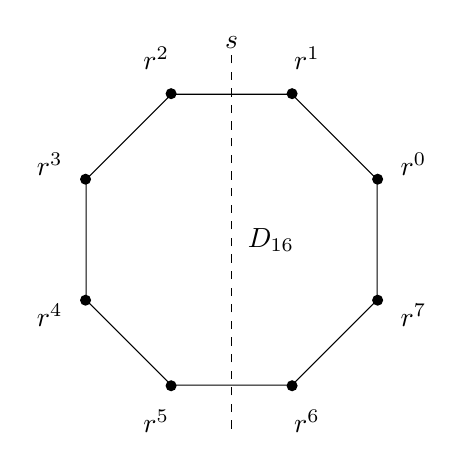
\begin{tikzpicture}
    \def\n{8} % number of sides
    \pgfmathtruncatemacro\dn{2*\n} % 2n for dihedral group
    \def\angle{360/\n} % angle of each sector
    \def\radialdist{2.5} % radial distance for labels
    \def\angleadjust{\angle/2} % angular shift to move label closer to vertex
    \node[regular polygon, regular polygon sides=\n, minimum size=4cm, draw] (poly) {};
  
    % Draw vertices
    \foreach \i in {1,2,...,\n} {
      \fill (poly.corner \i) circle[radius=2pt];
    }
    
    % Draw vertical line of symmetry
    \draw[dashed] (0,-2.4) -- (0,2.4);
    \node at (0,2.5) {$s$};

    % Labels for rotations
    \foreach \i [count=\xi starting from 0] in {1,2,...,\n} {
      \node at ({\i*\angle-\angleadjust}:{\radialdist}) {\(r^{\xi}\)};
    }

    % Label the dihedral group, moved to the side
    \node at (0.5,0) {\(D_{\dn}\)};
  \end{tikzpicture}
\end{figure}


\mprop{}{\begin{enumerate}
    \item $|r| = n$
    \item $|s| = 2$
    \item $s \neq r^i$ for any $i$
    \item $D_{2n} = \{1, r, r^2, \dots , r^{n-1} , s, sr, sr^2, \dots, sr^{n-1} \}$
    \item $rs = sr^{-1}$ (which shows that $D_{2n}$ is not abelian)
    \item $r^i = sr^{-i}$
\end{enumerate}}
For a group $G$, $S \subseteq G$ with the property that every element of $G$ can be written as as (finite) product of elements in $S$ and their inverses is a set of generators of $G$ ($S$ generates $G$). The equations that the generators satisfy are called relations (in $G$). For some collection of relations, $R_1 , R_2 , \dots , R_m$ such that the relation among any element can be deduced, the presentation of $G$ is written
$$G = \langle S \mid R_1, R_2, \dots, R_m \rangle$$
\ex{Presentation of Dihedral Group}{The presentation of Dihedral group of order $2n$ is $$D_{2n} = \langle r,s \mid r^n = s^2 = 1, rs = sr^{-1}\rangle$$}

\section{Symmetric Groups}
\dfn{Set of all Permutations}{Let $\Omega$ be any nonempty set. $S_\Omega$ is the set of all permuations of $\Omega$. It is denoted $S_n$ in the special case when $\Omega = \{1, 2, \dots, n$\}.}
Under function composition, $S_\Omega$ is called the symmetric group on the nonemptyset $\Omega$. For symmetric groups, we now use cycle decomposition notation, which is much more efficient. If $a_i \mapsto a_{i+1}$ for $1 \leq i \leq m-1$ and $a_m \mapsto a_1$, with $k$ cycles, we write $$(a_1 \hspace{4pt} a_2 \hspace{4pt}\dots \hspace{4pt} a_{m_1})(a_{m_1 +1} \hspace{4pt} a_{m_1 +2} \hspace{4pt}\dots \hspace{4pt} a_{m_2})\dots(a_{m_{k-1}+1} \hspace{4pt} a_{m_{k-1}+2} \hspace{4pt}\dots \hspace{4pt} a_{m_k})$$
The length of a cycle is the number, $t$, of integers appearing in it, called a $t-cycle$. Two cycles are disjoint if they have no numbers in common. Elements that are mapped to themselves aren't written in cycle decomposition. 
\nt{Since the binary operation is function composition, the product of two cycles $(1 \hspace{4pt} 2) \circ (2 \hspace{4pt} 3)$, shortened to $(1 \hspace{4pt} 2) (2 \hspace{4pt} 3)$ when the context is clear, is equal to $(1 \hspace{4pt} 2 \hspace{4pt} 3)$ since function composition is read right to left.}

\section{Matrix Groups}
\dfn{Field}{A field is a set $F$ under two binary operations $+$ and $\cdot$ such that $(F, +)$ and $(F-\{0\}, \cdot)$ are an abelian groups following the distributive law:
$$\forall a,b,c \in F, a\cdot(b+c) = (a \cdot b) + (a \cdot c)$$
Let $F^\times = F - \{0\}$ for any field $F$.}
\ex{Fields}{A few examples of fields include\begin{itemize}
    \item $\bbQ$
    \item $\bbR$
    \item For a prime $p$, $\bbZ / p\bbZ$, which will be denoted $\bbF_p$
\end{itemize}}
\dfn{General Linear Group of Degree $n$}{Let $M_{n \times n}$ be the set of all $n \times n$ matrices. For any $n \in \bbZ^+$, $$\GL_n (F) = \{A \in M_{n \times n} \mid \det (A) \neq 0 \}$$}
The order of a finite field is equal to $p^m$ for some prime $p$ and integer $m$. Additionally, for a field $F$, 
$$|F| = q < \infty \implies |\GL_n(F)|=\prod_{m=0}^{n-1} (q^n -q^m)$$

\section{The Quaternion Group}
\dfn{The Quaternion Group}{The quaternion group, \( Q_8 \), is defined by
\begin{align*}
Q_8 &= \{1, -1, i, -i, j, -j, k, -k\}
\end{align*}
with product \(\cdot\) computed as follows: For all $a \in Q_8$, $$1 \cdot a = a \cdot 1 =a$$
$$(-1) \cdot (-1) = 1$$
$$(-1) \cdot a = a, a\cdot (-1) = -a$$
$$i \cdot i = j \cdot j = k \cdot k = -1 $$
\begin{align*}
i \cdot j &= k, & j \cdot i &= -k \\
j \cdot k &= i, & k \cdot j &= -i \\
k \cdot i &= j, & i \cdot k &= -j.
\end{align*}}

\section{Homomorphisms and Isomorphisms}
\dfn{Homomorphism}{Let $(G,*)$ and $(H, \cdot)$ be groups. A homomorphism is a map $\varphi : G \rightarrow H$ such that $$\forall x,y \in G, \varphi (x * y) = \varphi(x)\cdot\varphi(y)$$}
\dfn{Isomorphism}{An isomorphism is a bijective homomorphism. Two isomorphic groups $G$ and $H$ can be written $G \cong H$.}
\ex{Isomorphisms}{\begin{itemize}
    \item The identity map is an obvious isomorphism.
    \item $\exp : \bbR \rightarrow \bbR^+$ is an isomorphism from $(\bbR, +)$ to $(\bbR^+,\times)$.
\end{itemize}}
It is easy to see if two groups are not isomorphic. For an isomorphism $\varphi : G \rightarrow H$, 
\begin{align*}
    &{\vcenter{\hbox{\tiny$\bullet$}}} \hspace{2pt} |G|=|H| \\
    &{\vcenter{\hbox{\tiny$\bullet$}}} \hspace{2pt} G\text{ is abelian if and only if $H$ is abelian}\\
    &{\vcenter{\hbox{\tiny$\bullet$}}} \hspace{2pt} \forall x \in G, |x| = |\varphi(x)|\\
\end{align*}
\section{Group Actions}
\dfn{Group Action}{A group action of a group $G$ on a set $A$ is a map from $G \times A$ to $A$, written as $g \cdot a$ for all $g \in G$ and $a \in A$, that satisfies the following properties:
\begin{enumerate}
    \item $\forall g_1 , g_2 \in G, a \in A, g_1 \cdot (g_2 \cdot a) = (g_1 g_2)\cdot a$, and 
    \item $\forall a \in A, 1 \cdot a = a.$
\end{enumerate}}
\nt{We say that $G$ is a group acting on a set $A$.}
Let the group $G$ act on the set $A$. For each fixed $g \in G$, we get a map $\sigma_g : A \rightarrow A$ defined by 
$$\sigma_g (a) = g \cdot a.$$
\mprop{}{\begin{enumerate}
    \item For each fixed $g \in G$, $\sigma_g$ is a permutation of $A$, and 
    \item The map from $G$ to $S_A$ defined by $g \mapsto \sigma_g$ is a homomorphism (and it is called the permutation representation associated to the given action).
    \end{enumerate}} 
\begin{myproof}
    \begin{enumerate}
        \item $\sigma_g$ is a map from $A$ to $A$, and it can be shown to be a permutation if it is bijective (and has a two-sided inverse).     
        \begin{align*}
            (\sigma_{g^{-1}}\circ \sigma_g)(a) &= \sigma_{g^{-1}}(\sigma_g (a))\\
            &=g^{-1}\cdot(g \cdot a)\\
            &=(g^{-1}g)\cdot a\\
            &=1\cdot a=a
        \end{align*}
        Then $\sigma_{g^{-1}} \circ \sigma_g : A \rightarrow A$ is the identity map. $g$ was arbitrary and we can interchange the roles of $g$ and $g^{-1}$ to obtain $\sigma_g \circ \sigma_{g^{-1}}$ is also the identity map. Then, $\sigma_g$ has a two-sided inverse, hence is a permuatation of $A$. 
        \item Let $\varphi: G \rightarrow S_A$ be defined by $g \mapsto \sigma_g$ (and note that we just proved $\sigma_g \in S_A$). For all $a \in A$,
        \begin{align*}
            \varphi(g_1 g_2)(a) &= \sigma_{g_1 g_2}(a)\\
            &=(g_1 g_2)\cdot a\\
            &=g_1\cdot (g_2 \cdot a)\\
            &=\sigma_{g_1}(\sigma_{g_2} (a))\\
            &=(\varphi(g_1)\circ \varphi(g_2))(a)
        \end{align*}
        Thus, $\varphi$ is a homomorphism. 
    \end{enumerate}
\end{myproof}

\chapter{Subgroups}
\section{Definitions}
\dfn{Subgroup}{Let $G$ be a group. $H \subseteq G$ is a subgroup of $G$ if $H \neq \emptyset$ and 
$$x,y \in H \implies x^{-1} \in H, xy \in H$$
$H \leq G$ denotes that $H$ is a subgroup of $G$. $H < G$ denotes proper containment.}
If $G$ is a group and $H \leq G$, $H$ has the same binary operation on $G$ and is a group. 
\ex{Subgroups}{\begin{itemize}
    \item $\bbZ \leq \bbQ$ and $\bbQ \leq \bbR$ under addition.
    \item All groups have trivial subgroup $\{1\}$ called the trivial subgroup, henceforth denoted by 1.
    \item Let $H = \{1, r, r^2, \dots , r^{n-1} \}$. $H$ is closed under the binary operation of $D_{2n}$ and $H \subseteq D_{2n}$ so $H \leq D_{2n}$.
    \item The set of all even integers is a subgroup of $\bbZ$ under addition.
\end{itemize}}
\mprop{The Subgroup Criterion}{Let $G$ be a group. $H \subseteq G$ is a subgroup if and only if
\begin{enumerate}
    \item $H \neq \emptyset$
    \item $\forall x, y \in H, xy^{-1} \in H$. 
\end{enumerate}}
\begin{myproof}
    1. and 2. must obviously hold if $H \leq G$.\\
    To show that the converse holds, let $x \in H$ (since $H \neq \emptyset$). Letting $y =x$ implies that $xx^{-1} \in H$, so $ 1 \in H$. \\
    Then, $H$ must contain the elements 1 and $x$, so it must also contain $1x^{-1}$ and $x^{-1} \in H$, implying that $H$ is closed under taking inverses.\\
    Finally, if $x,y,y^{-1} \in H \implies  x(y^{-1})^{-1}\in H$. Then, $xy \in H$. Hence, $H$ is a subgroup of $G$. 
\end{myproof}
\section{Centralizers, Normalizers, Stabilizers, and Kernels}
\dfn{Centralizer}{The centralizer of nonempty $A\subseteq G$ in group $G$ is the subset of $G$
$$C_G (A) = \{ g \in G \mid \forall a \in A,  gag^{-1} =a\}$$
$C_G(A)$ contains all elements of $G$ that commute with every element in $A$.}
To show that $C_G (A) \leq G$, we first see that $1 \in C_G (A) \implies G_G \neq \emptyset$. Secondly, assume that $x, y \in C_G(A)$, or 
$$\forall a \in A, xax^{-1} = a, yay^{-1} = a$$
\begin{align*}
    (xy)a(xy)^{-1} &= (xy)a(y^{-1} x^{-1}) \\
    &= x(yay^{-1})x^{-1} \\
    &= xax^{-1} \\
    &= a 
\end{align*}
Then, $x, y \in C_G(A) \implies xy \in C_G(A)$. Observe that $xax^{-1} = a \implies  a = x^{-1}ax$ so $\forall x \in C_G(A), x^{-1} \in C_G(A)$. Therefore, $C_G(A)$ is a subgroup. 
\ex{Centralizers of Groups}{\begin{itemize}
    \item If $G$ is an abelian group, $\forall A \subseteq G, C_G(A) = G$
    \item $C_{Q_8} (i) = \{\pm 1, \pm i\}$
\end{itemize}}
\dfn{Center}{The center of $G$ is the subset 
$$Z(G) = C_G(G) = \{ g \in G \mid  \forall x \in G, gx=xg\}$$
This is the set of all elements commuting with all elements of $G$. }
\dfn{Normalizer}{Define 
$$gAg^{-1} = \{gag^{-1} \mid a \in A\}.$$
The normalizer of $A$ in $G$ is the set 
$$N_G(A) =\{g \in G \mid gAg^{-1} = A\}.$$}
If $G$ is a group acting on set $S$, for some fixed $s \in S$ the stabilizer of $s$ in $G$ is the set 
$$G_s = \{g \in G \mid g \cdot s = s \}$$
%insert proof that G_s is a subgroup of G. 
The kernel of the action of $G$ on $S$ is defined as 
$$\{g \in G \mid \forall s \in S,  g \cdot s = s\}$$
%insert similar subgroup proof
\section{Cyclic Groups and Cyclic Subgroups}
\dfn{Cyclic Group}{A group $H$ is cyclic if 
$$\exists x \in H, H = \{x^n \mid n \in \bbZ \}$$
Equivalently, $H$ is cyclic if it can be generated by a single element. }
Observe that $H = \langle x \rangle \implies H = \langle x^{-1} \rangle$. Additionally, note that all cyclic groups are abelian. 
\mprop{}{$$H = \langle x \rangle \implies |H| = |x|$$
(one side being infinite implies that the other is too.)\\
More specifically, 
\begin{enumerate}
    \item $|H| = n < \infty \implies x^n = 1$ and $1, x, x^2, \dots , x^{n-1}$ are all distinct elements in $H$
    \item $|H| = \infty \implies (\forall n \neq 0, x^n \neq 1) \land (\forall a \neq b \in \bbZ, x^a \neq x^b)$
\end{enumerate}}
\iffalse
\begin{myproof}
    Let $|x| = n$ and consider the $n < \infty$ case. Suppose for $0 \leq a < b < n$, $x^a = x^b$. Then, $x^{b-a} = 1$, yielding a contradiction since $n$ is the smallest positive power of $x$ giving the identity. 
\end{myproof}
\fi
\mprop{}{Let $G$ be an arbitrary group, $x\in G$, and $m, n \in Z$. 
$$x^n = 1 \land x^m = 1 \implies x^{(m,n)} = 1.$$
In particular, 
$$x^m = 1 \implies (|x|) \mid m.$$}
\begin{myproof}
    By the Euclidean Algorithm, $\exists r,s \in \bbZ, (m, n) = mr + ns$. Thus, 
    $$x^{(m,n)} = x^{mr+ns} = (x^m)^r (x^n)^s = 1^r 1^s = 1.$$
\end{myproof}
\thm{Cyclic Group Isomorphism}{\begin{enumerate}
    \item If $n \in \bbN$ and $\langle x \rangle$ and $\langle y \rangle$ are both cyclic groups of order $n$, there exists a well defined isomorphism
    $$\varphi : \langle x\rangle \to \langle y \rangle$$
    $$x^k \mapsto y^k$$
    \item If $\langle x \rangle$ is an infinite cyclic group, there exists a well defined isomorphism
    $$\varphi : \bbZ \to \langle x \rangle$$
    $$k \mapsto x^k$$
\end{enumerate}}
\begin{myproof}
    Let $\langle x \rangle $ and $\langle y \rangle$ be cyclic groups of order $n$ and $\varphi: \langle x \rangle \to \langle y \rangle, x^k \mapsto y^k$. To prove $\varphi$ is well defined ($x^r = x^s \implies \varphi (x^r) = \varphi (x^s)$), $x^{r-s} = 1$ so, by proposition 2.3.2, $n \mid r - s$. Then, 
    \begin{align*}
        r &= tn + s\\
        \varphi(x^r) &= \varphi (x^{tn+s})\\
        & = y^{tn+s}\\
        &= (y^n)^t y^s\\
        &= y^s = \varphi (x^s)
    \end{align*}
    
    Thus, $\varphi$ is well defined. $\varphi (x^a x^b) = \varphi(x^a) \varphi(x^b)$ so $\varphi$ is a homomorphism. All elements $y^k$ have a preimage $x^k$ so the map is surjective. The groups have the same finite order so $\varphi$ must be bijective if it is a surjection. Thus, $\varphi$ is an isomorphism. 
    If $\langle x \rangle$ has infinite order, let well defined map $\varphi : \bbZ \to \langle x \rangle , k \mapsto x^k$. $\forall a \neq b \in \bbZ, x^a \neq x^b$ so it is injective. $\varphi$ is surjective by the definition of a cyclic group. Then, $\varphi$ is an isomorphism. 
    
    Now, let $\langle x \rangle$ be an infinite cyclic group, and $\varphi : \bbZ \to \langle x \rangle , k \mapsto x^k$. $\varphi$ is obviously well defined, and since $a \neq b \implies x^a \neq x^b$, $\varphi$ is injective. $\varphi$ is surjective by the definition of a cyclic group, and it can be verified to be a homomorphism. Thus, $\varphi$ is an isomorphism. 
\end{myproof}
From now on, let for each $n \in \bbN$, let $Z_n$ denote the cyclic group of order $n$, written multiplicatively. 
\mprop{}{Let $G$ be a group, $x \in G$, $a \in \bbZ - \{ 0 \}$
\begin{enumerate}
    \item $|x| = \infty \implies | x^a | = \infty$
    \item $|x | = n < \infty \implies |x^a| = \frac{n}{(n,a)}$
    \item $|x| = n < \infty \land (a \in \bbZ^+, a \mid n) \implies |x^a| = \frac{n}{a}$
\end{enumerate}}
\begin{myproof}
    Suppose that $|x| = \infty$ but $|x^a | = m < \infty$. By the definition of order,
    $$1 = (x^a)^m = x^{am}$$
    $$x^{-am} = (x^{am})^{-1} =1$$
    Either $am$ is positive or $-am$ is, so there exists a positive power of $x$ equal to the identity, which is a contradiction. 

    Let $y = x^a, (n,a) = d, n = db, a = dc$ for $b,c \in \bbZ, b> 0$. $d$ is the gcd of $n$ and $a$ so $(b,c) = 1$. To show that $|y| = b$, 
    $$y^b = x^{ab} = x^{dcb} = (x^n)^c = 1$$
    so $(|y|) \mid b$. Then, 
    $$x^{a|y|} = y^{|y|} = 1$$
    It follows that $n \mid (a|y|)$ so $b \mid (c |y|)$. $(b,c) = 1$ so $b \mid (|y|)$. $b \mid (|y|)$ and $(|y|) \mid b$ implies that $|y| = b$. Thus, $n = d|y|$ and $|y| = \frac{n}{d}$
\end{myproof}
\mprop{}{Let $H = \langle x \rangle$. 
\begin{enumerate}
    \item $|x| = \infty \implies (H = \langle x^a \rangle \iff a = \pm 1$)
    \item $|x| = n < \infty \implies (H = \langle x^a \rangle \iff (a, n ) = 1$). Note that the number of generators of $H$ is $\varphi (n)$ (where $\varphi$ is Euler's $\varphi$-function)
\end{enumerate}}
\begin{myproof}
    If $|x| = n < \infty,$ $x^a$ generates a subgroup of $H$ of order $|x^a|$. This subgroup equals $H$ if and only if $|x^a| = |x|$. 
    $$|x^a| = |x| \iff \frac{n}{(a,n)} = n$$
    Then $(a,n) = 1$, and by definition $\varphi (n)$ is the number of such generators.  
\end{myproof}
\thm{}{Let $H = \langle x \rangle$ be a cyclic group. 
\begin{enumerate}
    \item $K \leq H \implies (K = \{1\}) \lor (K = \langle x^d \rangle)$, where $d$ is the smallest positive integer such that $x^d \in K$.
    \item $|H| = \infty \implies \forall a \neq b \in \bbN, \langle x^a \rangle \neq \langle x^b \rangle$. Additionally, $\forall m \in \bbZ , \langle x^m \rangle = \langle x^{|m|} \rangle$, so the nontrivial subgroups of $H$ correspond bijectively with $\bbN$. 
    \item $|H | = n < \infty$ implies that for each $a \in \bbN, a | n$ there is a unique subgroup of $H$ of order $a$, $\langle x^d \rangle , d = \frac{n}{a}$. Furthermore, for every integer $m$, $\langle x^m \rangle = \langle x^{(n,m)} \rangle$, so the subgroups of $H$ correspond bijectively with the positive divisors of $n$. 
\end{enumerate}}
\begin{myproof}
    Let $K \leq H$. The proposition is true for $K = \{1\}$, so assume $K \neq \{1\}$. Thus, $\exists a \neq 0, x^a \in K$. 
    $$a < 0 \implies x^{-a} = (x^a)^{-1} \in K$$
    so $K$ always contains a positive power of $x$. Let 
    $$\mcP = \{ b \mid b \in \bbZ^+ \land x^b \in K \}$$
    There must exist a minimum element $d \in \mcP$. $K$ is a subgroup and $x^d \in K$ so $\langle x^d \rangle \leq K$. $K \leq H$ so any element in $K$ is of the form $x^a$ for some integer $a$. 
    $$a = qd + r, \hspace{10pt} 0 \leq r < d$$
    $$x^r = x^a (x^d) ^{-q} \in K$$
    since both $x^a, x^d \in K$. By minimality of $d$, $r = 0$ so $x^a = (x^d)^q \in \langle x^d \rangle$. Thus, $K \leq \langle x^d \rangle$, and since $\langle x^d \rangle\leq K$,  $\langle x^d \rangle = K$

    Assume $|H| = n < \infty$ and $a \mid n$. Let $d = \frac{n}{a}$ so $\langle x^d \rangle$ so is a subgroup of order $a$, showing its existence. To show uniqueness, suppose $K$ is any order $a$ subgroup of $H$, with 
    $$K = \langle x^b \rangle$$
    for the minimum positive integer $b$ such that $x^b \in K$. 
    $$\frac{n}{d} = a = |K| = |x^b| = \frac{n}{(n,b)}$$
    so $d = (n,b)$ and $d \mid b$. Then, $x^b \in \langle x^d \rangle$, hence 
    $$K \leq \langle x^d \rangle$$
    $| \langle x^d \rangle | = a = |K|$ so $K = \langle x^d \rangle$. $\langle x^m \rangle$ and $\langle x^{(n,m)} \rangle $ have the same order and $(n, m) \mid n$. Thus, $\langle x^m \rangle = \langle x^{(n,m)} \rangle$
\end{myproof}
%insert proof
\chapter{Quotient Groups and Homomorphisms}
\section{Definitions}
\dfn{Kernel}{The kernel of homomorphism $\varphi : G \to H$ is the set 
$$\ker \varphi = \{ g \in G \mid \varphi(g) = 1 \}$$}
\mprop{}{Let $G$ and $H$ be groups and $\varphi : G \to H$ be a homomorphism.
\begin{enumerate}
    \item $\varphi (1_G) = 1_H$ ($1_G$ and $1_H$ are identities of $G$ and $H$, respectively)
    \item $\forall g \in G, \varphi(g^{-1}) = \varphi(g)^{-1}$
    \item $\forall n \in \bbZ, \varphi(g^n) = \varphi(g)^n$
    \item $\ker \varphi \leq G$
    \item The image of $G$ under $\varphi$, $\img (\varphi) \leq H$
\end{enumerate}}
\dfn{Quotient Group}{Let $\varphi : G \to H$ be a homomorphism with kernel $K$. The quotient group, $G/K$ (read $G$ modulo $K$) is the group whose elements are fibers (set of preimages) of $\varphi$, with group operation such that if $X$ and $Y$ are the fibers above $a$ and $b$ respectively, the product of $X$ and $Y$ is the fiber above the product $ab$. }
\mprop{}{Let $\varphi : G \to H$ be a homomorphism of groups with kernel $K$. Let $X = \varphi^{-1} (a)$. Then, 
\begin{enumerate}
    \item $\forall u \in X, X = \{uk \mid k \in K \}$
    \item $\forall u \in X, X = \{ku \mid k \in K \}$
\end{enumerate}}
\begin{myproof}
    Let $u \in X$. By definition of $X$, $\varphi (u) = a$. Let 
    $$uK = \{ uk \mid k \in K \}$$
    To prove $uK \subseteq X$, 
    \begin{align*}
        \forall k \in K, \varphi(uk) &= \varphi(u)\varphi(k)\\
        &= \varphi(u)1\\
        &= a
    \end{align*}
    so $uk \in X \implies uK \subseteq X$. To prove the reverse inclusion, let $g \in X$ and $k = u^{-1} g$. 
    $$\varphi(k) = \varphi(u^{-1} )\varphi(g) = \varphi(u)^{-1} \varphi (g)$$
    $$= a^{-1} a = 1$$
    So $k \in \ker \varphi$, and $g = uk \in uK$, establishing $X \subseteq uK$. Therefore, $X = uK$. 
\end{myproof}
\dfn{Coset}{For any $N \leq G$ and $g \in G$, 
$$gN = \{gn \mid n \in N \} \text{  and  } Ng = \{ ng \mid n \in N \}$$
are the left and right cosets of $N$ in $G$, respectively. Any element of a coset is called a representative for it.}
\thm{}{Let $G$ be a group and $K$ be the kernel of some homomorphism from $G$ to another group. The set of left cosets of $K$ in $G$ with operation defined by 
$$uK \circ vK = (uv)K$$
forms a group, $G/K$. This operation is well defined in the sense that $u_1 \in uK \land v_1 \in vK \implies u_1 v_1 \in uvK$. Additionally, $u_1 v_1 K = uvK$ so the multiplication doesn't depend on choice of representatives (element in coset) for the cosets. This statement is true when ``left coset" is interchanged ``right coset."}
\begin{myproof}
    Let $X,Y \in G/K$ and $Z = XY \in G/K$ (by definition). Then, $X,Z,$ and $Z$ are (left) cosets of $K$. Assume $K$ is the kernel of some homomorphism $\varphi : G \to H$ so $X = \varphi ^{-1} (a)$ and $Y = \varphi^{-1} (b)$ for some $a,b \in H$. By the definition of the $G/K$ operation, $Z = \varphi^{-1} (ab)$. Let $u \in X$ and $v \in Y$ be arbitrary representatives their cosets, so $\varphi (u) = a, \varphi(v) = b, X = uK, Y = vK$. 
    \begin{align*}
        uv \in Z &\iff uv \in \varphi^{-1} (ab)\\
        & \iff \varphi(uv) = ab\\
        & \iff \varphi(u)\varphi(v) = ab
    \end{align*}
    The latter equality holds so $uv \in Z \implies Z = uvK$. Thus, $XY = uvK$ for any representatives $u \in X, v \in Y$. The last statement follows since $\forall u \in G, uK=Ku$.
\end{myproof}
It is important to note that multiplication is independent of the representative chosen. $\overline{u}$  can be used to denote a coset $uK$, and $\overline{G}$ can denote $G/K$. Then, $\overline{u} \cdot \overline{v} = \overline{uv}$. 
\ex{}{\begin{itemize}
    \item If $\varphi : G \to H$ is an isomorphism, $K = 1$ and the fibers of $\varphi$ each contain one element, so $G/1 \cong G$.
    \item Let $G$ be any group and $H = 1$ be a group of order 1. $\varphi: G \to H, g \in G \mapsto 1$ is the trivial homomorphism. $\ker \varphi = G$ and $G/G \cong Z_1 = \{1\}.$
    \item Define $\varphi : Q_8 \to V_4$ by $$\pm 1 \mapsto 1,\hspace{5 pt} \pm i \mapsto a,\hspace{5 pt} \pm j \mapsto b, \hspace{5 pt} \pm k \mapsto c$$
    $\ker \varphi = \{\pm 1 \}$ and $Q_8 / \langle \pm 1 \rangle$ can be thought of as the ``absolute value" of $Q_8$. 
\end{itemize} }
\mprop{}{Let $N \leq G$. The set of left cosets of $N$ in $G$ form a partition of $G$. Additionally, $$\forall u,v \in G, uN = vN \iff v^{-1} u \in N$$
$$uN = vN \iff u \in vN \land v \in uN$$}
\begin{myproof}
    $$N \leq G \implies 1 \in N$$
    $$\forall g \in G, g = g\cdot 1 \in gN$$
    $$G = \bigcup_{g \in G} gN$$
    To show that $uN \cap vN \neq \emptyset$, let $x \in uN \cap vN$, for some $n,m \in N$, 
    $$x = un = vm$$
    $$u = vmn^{-1} = vm_1$$
    $$\forall ut \in uN, ut = (vm_1)t = v(m_1 t) \in vN.$$
    Thus, $uN \subseteq vN$. $u$ and $v$ can be interchanged to obtain that $vN \subseteq uN$. Therefore, $uN \cap vN \neq \emptyset \implies uN = vN$.  
    $$uN = vN \iff u \in vN \iff n \in N, u =vn \iff v^{-1} u \in N$$
\end{myproof}
\mprop{}{Let $G$ be a group and $N \leq G$. 
\begin{enumerate}
    \item The operation described by 
    $$uN \cdot vN = (uv) N$$
    is well defined if and only if $\forall g \in G, n \in N, gng^{-1} \in N$. 
    \item If the operation is well defined then the set of left cosets of $N$ in $G$ is a group. The identity is $1N$ and $(gN)^{-1} = g^{-1}N.$
\end{enumerate}}
\begin{myproof}
    First assume $$\forall u,v \in G, u,u_1 \in uN \land v,v_1 \in vN \implies uvN = u_1 v_1 N.$$
    Let $g \in G$ and $n \in N$. If $u = 1, u_1 = n, v = v_1 = g^{-1}$ then 
    $$1g^{-1} N = ng^{-1} N$$
    $$1 \in N \implies ng^{-1} \cdot 1 \in ng^{-1} N$$
    $$ng^{-1} \in g^{-1} N \implies ng^{-1} = g^{-1}n_1$$
    for some $n_1 \in N$. Thus, $gng^{-1} = n_1 \in N$. Now assume $\forall g \in G, n \in N, gng^{-1} \in N$. Let $u,u_1 \in uN$ and $v,v_1 \in vN$. For some $n,m \in N$, 
    $$u_1 = un$$
    $$v_1 = vm$$
    To prove $u_1 v_1 \in uvN$, 
    \begin{align*}
    u_1 v_1 &= (un)(vm) = u(vv^{-1})nvm\\
    &= (uv)(v^{-1}nv)m = (uv)(n_1m)
    \end{align*}
    where $n_1 = v^{-1} n v \in N$. Now $N$ is closed under products so $n_1 m \in N$ and $u_1 v_1 = (uv)n_2$ for some $n_2 \in N$. Thus, $uvN$ and $u_1 v_1 N$ contain the common element $u_1 v_1$. 
\end{myproof}
\dfn{Normal Subgroup}{$gng^{-1}$ is the conjugate of $n \in N$ by $g$. $gNg^{-1} = \{gng^{-1} \mid n \in N\}$ is the conjugate of $N$ by $g$. $g$ is said to normalize $N$ if $gNg^{-1} = N$. A subgroup $N$ of $G$ is said to be normal (denoted $N\unlhd G$) if $\forall g \in G, gNg^{-1} = N$.}
\thm{}{Let $N \unlhd G$. The following are equivalent:
\begin{enumerate}
    \item $N \unlhd G$
    \item $N_G (N) = G$
    \item $\forall g \in G, gN = Ng$
    \item The set of left cosets form a group under the operation described in proposition 3.1.4
    \item $\forall g \in G, gNg^{-1} \subseteq N$
\end{enumerate}}
\mprop{}{For some $N \leq G$ and homomorphism $\varphi$, $$N \unlhd G \iff N = \ker \varphi$$}
\begin{myproof}
    $N = \ker \varphi \implies \forall g \in G, gN = Ng$ so $N$ will be normal. Conversely, let $H = G/N$ and $\pi : G \to G/N$ defined by $\forall g \in G, g \mapsto gN$. 
    $$\pi (g_1 g_2) = (g_1 g_2)N = g_1N g_2 N = \pi(g_1)\pi(g_2)$$
    so $\pi$ must be a homomorphism. 
    \begin{align*}
    \ker \pi &= \{g \in G \mid \pi (g) = 1N \}\\
    &= \{g \in G \mid gN = 1N \}\\
    &= \{g \in G \mid g \in N \} = N
    \end{align*}
\end{myproof}
\dfn{Natural Projection}{Let $N \unlhd G.$ The homomorphism $\pi :G \to G/N$ defined by $g \mapsto gN$ is called the natural projection (homomorphism) of $G$ onto $G/N$. If $\overline H \leq G/N$, the complete preimage of $\overline H$ in $G$ is the preimage of $\overline H$ under the natural projection homomorphism.}
\ex{}{Let $G$ be a group
\begin{itemize}
    \item $G/1 \cong G, \hspace{10pt} G/1 \unlhd G$\\ $G/G \cong 1 , \hspace{10pt} G/G \unlhd G$
    \item If $G$ is abelian, $\forall N \leq G, N \unlhd G$, because 
    $$\forall g \in G, n \in N, gng^{-1} = gg^{-1}n = n \in N$$
    Note that only $N$ being abelian is not sufficient. \\Suppose $G = Z_k$. Let $x$ be a generator of $G$ and $N \leq G$. $N = \langle x^d \rangle$, where $d$ is the smallest power of $x$ that lies in $N$. 
    $$G/N = \{gN \mid g \in G\} = \{ x^{\alpha} \mid \alpha \in \bbZ \}$$
    and since $x^\alpha N= \langle xN \rangle ^\alpha$, $G/N = \langle xN \rangle$. $$|xN| =d = \frac{|G|}{|N|}.$$ 
    Thus, quotient groups of a cyclic group are cyclic. 
    \item Generalizing the previous example, $N \leq Z(G) \implies N \unlhd G$. 
\end{itemize}}
\section{Lagrange's Theorem}
\thm{Lagrange's Theorem}{If $G$ is a finite group and $H \leq G$, $|H|\hspace{2pt} \big| \hspace{2pt} |G|$, and the number of left cosets of $H$ in $G$ equals $|G| / |H|$.}
\begin{myproof}
    Let $|H| = n$ and let the number of left cosets of $H$ in $G$ equal $k$. The set of left cosets of $H$ in $G$ partition $G$. The map 
    $$H \to gH \text{\hspace{10pt} defined by \hspace{10pt}} h \mapsto gh$$
    is surjective. This map is injective because $gh_1 = gh_2 \implies h_1 = h_2$. Thus, 
    $$|gH| = |H| = n.$$
    $G$ is partitioned into $k$ disjoint subsets each with cardinality $n$, so $|G| = kn$. Thus, 
    $$k = \frac{|G|}{n} = \frac{|G|}{|H|}.$$
\end{myproof}
\dfn{Index}{If $G$ is a group and $H \leq G$, the number of left cosets of $H$ in $G$ is called the index of $H$ in $G$, denoted by $|G: H|$.}

\cor{}{If $G$ is a finite group and $x \in G$, $|x|\hspace{2pt} \big| \hspace{2pt} |G|$. In particular, $\forall x \in G, x^{|G|} = 1$}
\cor{}{If $|G| = p$ for some prime $p$, then $G$ is cyclic, hence $G \cong Z_p$.}
\begin{myproof}
    Let $x \in G, x \neq 1$. Thus $| \langle x \rangle | > 1$, and $| \langle x \rangle |$ divides $|G|$. $|G|$ is prime so $|\langle x \rangle | = |G|$. Thus, $G = \langle x \rangle$.
\end{myproof}

%insert examples

\thm{Cauchy's Theorem}{If $G$ is a finite group and a prime $p$ divides $|G|$, then $G$ has an element of order $p$.}
\thm{Sylow}{If $G$ is a finite group of order $p^\alpha m$, where $p$ is prime and $p \nmid m$, then $G$ has a subgroup of order $p^\alpha$.}
\dfn{}{Let $H$ and $K$ be subgroups and define 
$$HK = \{hk \mid h \in H, k \in K \}$$}
\mprop{}{If $H$ and $K$ are finite subgroups of a group then 
$$|HK| = \frac{|H||K|}{|H \cap K|}$$}
\begin{myproof}
    $$HK = \bigcup_{h \in H} hK.$$
    Each coset of $K$ has $|K|$ elements. To find the number of distinct left cosets, $h_1 K = h_2 K \iff h_2 ^{-1} h_1 \in K$. Thus, 
    $$h_1 K = h_2 K \iff h_2 ^{-1}h_1 \in H \cap K \iff h_1 ( H \cap K) = h_2 (H \cap K).$$
    Thus the number of distinct cosets of the form $hK$ for $h \in H$ is the number of distinct cosets $h(H \cap K)$ for $h \in H$. By Lagrange's Theorem, this is $|H|/|H\cap K |$. Thus $HK$ consists of $|H|/|H\cap K|$ distinct cosets of $K$, each with $|K|$ elements. 
\end{myproof}
\mprop{}{If $H \leq G$ and $K \leq G$, $HK\leq G \iff HK = KH$}
\begin{myproof}
    First assume $HK = KH$ and let $a,b \in HK$. To prove $ab^{-1} \in HK$ so it is a subgroup, let 
    $$a = h_1 k_1 \text{\hspace{10pt} and \hspace{10pt}} b = h_2 k_2$$
    for some $h_1 ,h_2 \in H$ and $k_1 , k_2 \in K$. Thus, $b^{-1} - k_2 ^{-1} h_2 ^{-1}$, so $ab^{-1} = h_1 k_1 k_2^{-1}h_2^{-1}$. Let $k_3 = k_1 k_2 ^{-1} \in K$ and $h_3 = h_2 ^{-1}$. Thus $ab^{-1}=h_1 k_3 h_3$. Since $HK = KH$, 
    $$k_3 h_3 = h_4 k_4$$
    for some $h_4 \in H, k_4 \in K$. Thus $ab^{-1} = h_1 h_4 k_4$ and since $h_1 h_4 \in H, k_4 \in K$, $ab^{-1} \in HK$. \\
    Conversely, assume $HK \leq G$. Since $K \leq HK$ and $H \leq HK$, $KH \subseteq HK$ by the closure property of subgroups. Let $hk \in HK$. Since $HK$ is a subgroup, if $hk = a^{-1}$ and $a = h_1 K_1$,
    $$hk = (h_1 k_1)^{-1} = k_1 ^{-1} h_1^{-1} \in KH$$
    so $HK \subseteq KH$, implying $KH = HK$. 
\end{myproof}
\cor{}{If $H \leq G, K \leq G$, then $H \leq N_G (K) \implies HK \leq G$. In particular,
$$\forall H \leq G, K \unlhd G \implies HK \leq G$$}
\begin{myproof}
    To prove $HK = KH$, let $h \in H$, $k \in K$. $hkh^{-1} \in K$, hence 
    $$hk = (hkh^{-1}) h \in KH$$
    proving that $HK \subseteq KH$. Similarly, $kh = h(h^{-1} kh) \in HK$, so $HK = KH$. This corollary follows from the previous proposition. 
\end{myproof}
\dfn{}{If $A \subseteq N_G (K)$ (or $C_G (K)$), $A$ is said to normalize $K$ (or centralize $K$, respectively).}

\section{The Isomorphism Theorems}
\thm{The First Isomorphism Theorem}{For some homomorphism $\varphi : G \to H$, $$\ker \varphi \unlhd G \text{\hspace{10pt} and \hspace{10pt}} G/ \ker \varphi \cong \varphi(G).$$}
\cor{}{Let $\varphi : G \to H$ be a homomorphism
\begin{enumerate}
    \item $\varphi$ is injective if and only if $\ker \varphi = 1$
    \item $|G : \ker \varphi | = | \varphi (G)|.$
\end{enumerate}}
\thm{The Second/Diamond Isomorphism Theorem}{Let $G$ be a group $A \leq G$, $B \leq G$, and $A \leq N_G (B)$. Then, $AB 
\leq G$, $B \unlhd AB$, $A \cap B \unlhd A$, and $AB/G \cong A/A \cap B$. }
\begin{myproof}
    $AB$ is a subgroup of $G$ by corollary 3.2.3. Since $A \leq N_G (B)$ and $B \leq N_G (B)$, $AB \leq N_G (B)$ ($B \unlhd AB$). \\
    $B$ is normal in $AB$ so $AB/B$ is well defined. Define map $\varphi : A \to AB/B$ by $a \mapsto aB$. 
    $$\varphi(a_1 a_2 ) = (a_1 a_2)B = a_1 B \cdot a_2 B = \varphi(a_1) \varphi(a_2)$$
    From the definition of $AB$, $\varphi$ is surjective. The identity in $AB/B$ is coset $1B$ so $\ker \varphi$ consists of elements $a \in A$ with $aB = 1B$, which are the elements $a \in B$ ($\ker \varphi = A \cap B$). By the First Isomorphism Theorem, $A \cap B \unlhd A$ and $A/A \cap B \cong AB/B$. 
\end{myproof}
\thm{The Third Isomorphism Theorem}{Let $G$ be a group, $H \unlhd G$, $K \unlhd G$, and $H \leq K$. Then, $K/H \unlhd G/H$ and 
$$(G/H)/(K/H) \cong G/K$$
which can be denoted
$$\overline G / \overline K \cong G/K.$$}
\begin{myproof}
    Define 
    $$\varphi : G/H \to G/K$$
    $$(gH) \mapsto gK.$$
    To show $\varphi$ is well defined, suppose $g_1 H = g_2 H$. Then $g_1 = g_2$ for some $h \in H$. $H \leq K$ so $h \in K$, hence, $g_1 K = g_2 K$, or $\varphi(g_1 H) = \varphi (g_2 H)$. $g \in G$ can be chosen arbitrarily so $\varphi$ is surjective. Finally
    \begin{align*}
        \ker \varphi &= \{gH \in G/H \mid \varphi(gH) = 1K \}\\
        &= \{gH \in G/H \mid gK = 1K\} \\
        &= \{gH \in G/H \mid g \in K \} = K/H. 
    \end{align*}
    By the First Isomorphism Theorem, $(G/H)/(K/H) \cong G/K$. 
\end{myproof}
\thm{The Fourth/Lattice Isomorphism Theorem}{Let $G$ be a group and $N \unlhd G$. Then there is a bijection from the set of subgroups $A$ of $G$ which contain $N$ onto the set of subgroups $\overline A = A/N$ of $G/N$. In particular, every subgroup of $\overline G$ is of the form $A/N$ for some subgroup $A$ of $G$ containing $N$ (namely, its preimage in $G$ under the natural projection homomorphism from $G$ to $G/N$). This bijection have the following properties: $\forall A, B \leq G$, $N \leq A$, $N \leq B$,
\begin{enumerate}
    \item $A \leq B \iff \overline A \leq \overline B$
    \item $A \leq B \implies |B:A| = |\overline B : \overline A|$
    \item $\overline{\langle A, B \rangle} = \langle \overline A , \overline B \rangle$
    \item $\overline{A \cap B} = \overline A \cap \overline B$
    \item $A \unlhd G \iff \overline A \unlhd \overline G$. 
\end{enumerate}}

\section{Composition Series and The H\"{o}lder Program}
\mprop{}{If $G$ is a finite abelian group and a prime $p$ divides $|G|$, then $G$ contains an element of order $p$. }
\begin{myproof}
    We proceed by induction on $|G|$. $$|G| > 1 \implies \exists x \in G, x \neq 1$$
    By Lagrange's Theorem, 
    $$|G| = p \implies \exists x\in G , |x| = p$$
    and we are done. We may now assume $|G| > p$. Suppose $p$ divides $x$, so $|x| = pn$. 
    $$|x^n | = p$$
    and we have an element of order $p$ again, so we assume $p$ does not divide $|x|$. \\
    Let $N = \langle x \rangle$. $G$ is abelian so $N \unlhd G$. By Lagrange's Theorem, $|G/N| = \frac{|G|}{|N|}$
    and $|N| > 1$ so $|G/N| < |G|$. $p$ does not divide $|N|$ so $p$ must divide $|G/N|$. We can now apply the induction assumption to the smaller group $G/N$ to conclude it contains an element $\overline y = yN$ of order $p$. Since $y \notin N$ $(\overline y \neq \overline 1)$ but $y^p \in N$ $(\overline y^p = \overline 1)$, we must have $\langle y^p \rangle \neq \langle y \rangle$, or $|y^p | < |y|$. Then, $p$ divides $|y|$. We are now in the situation described in the preceding paragraph, which again produces an element of order $p$. 
\end{myproof}
\dfn{Simple}{A group $G$ is called simple if $|G| > 1$ and the only normal subgroups of $G$ are 1 and $G$. }
\dfn{Composition}{In a group $G$ a sequence of subgroups
$$1 = N_0 \leq N_1 \leq N_2 \leq \cdots \leq N_{k-1} \leq N_k = G$$
is called a composition series if $N_i \unlhd N_{i+1}$ and $N_{i+1}/N_i$ is a simple group, $0 \leq i \leq k-1$. If the sequence is a composition series, the quotient groups $N_{i+1}/N_i$ are called composition factors of $G$. }
\thm{Jordan-H\"older}{Let $G$ be a finite group with $G \neq 1$. Then
\begin{enumerate}
    \item $G$ has a composition series and 
    \item The composition factors in a composition series are unique, namely, if $1 = N_0 \leq N_1 \leq \cdots \leq N_r = G$ and $1 = M_0 \leq M_1 \leq \cdots \leq M_s = G$ are two composition series for $G$, then $r=s$ and there is some permutation, $\pi$, of $\{1, 2, \dots , r\}$ such that for $1 \leq i \leq r$,  
    $$M_{\pi (i)}/M_{\pi (i)-1} \cong N_i / N_{i-1}$$
\end{enumerate}}
\thm{}{There is a list consisting of 18 (infinite) families of simple groups and 26 simple groups not belonging to these families (the sporadic simple groups) such that every finite simple group is isomorphic to one of the groups in this list. }
\thm{Feit-Thompson}{If $G$ is a simple group of odd order, then $G \cong Z_p$ for some prime $p$. }
\dfn{Solvable}{A group $G$ is solvable if there is a chain of subgroups
$$1 = G_0 \unlhd G_1 \unlhd G_2 \unlhd \cdots \unlhd G_s = G$$
such that $G_{i+1}/G_i$ is abelian for $i = 0, 1, \dots , s-1$. }
\thm{}{The finite group $G$ is solvable if and only if for every divisor $n$ of $|G|$ such that $(n, \frac{|G|}{n} ) = 1$, $G$ has a subgroup of order $n$. }

\section{Transpositions and the Alternating Group}
\dfn{Transposition}{A 2-cycle is called a transposition.}
\dfn{Sign}{\begin{enumerate}
    \item $\eps(\sigma)$ is called the sign of $\sigma$
    \item $\sigma$ is called an even permutation if $\eps (\sigma)= 1$ and odd if $\eps(\sigma ) = -1$.
\end{enumerate}}

\mprop{}{The map $\eps : S_n \to \{\pm 1\}$ is a homomorphism (where $\{\pm 1\}$ is a multiplicative version of $Z_2$). }
\begin{myproof}
    Let $$\Delta = \prod_{1 \leq i < j \leq n} (x_i - x_j)$$
    then
    $$(\tau \sigma)(\Delta) = \prod_{1 \leq i < j \leq n} (x_{\tau \sigma (i)} - x_{\tau \sigma (j)})$$
    Suppose that $\sigma (\Delta)$ has exactly $k$ factors of the form $x_j -x_i$ with $j> i$, that is $\eps (\sigma) = (-1)^k$. When calculating $(\tau \sigma)(\Delta)$, after first applying $\sigma$ to the indices we see that $(\tau \sigma )(\Delta)$ has exactly $k$ factors of the form $x_{\tau (j)} - x_{\tau (i)}$ with $j>i$. Interchanging the order of the terms in these $k$ factors introduces the sign change $(-1)^k = \eps (\sigma)$, and now all factors of $(\tau \sigma)(\Delta)$ are of the form $x_{\tau(p)} - x_{\tau(q)}$, with $p< q$. Thus
    $$(\tau \sigma )(\Delta) = \eps (\sigma) \prod_{1 \leq p < q \leq n} (x_{\tau (p)} - x_{\tau (q)})$$
    By the definition of $\eps$, 
    $$\prod_{1 \leq p < q \leq n} (x_{\tau (p)} - x_{\tau (q)}) = \eps (\tau) \Delta$$
    We have $(\tau \sigma)(\Delta) = \eps(\sigma) \eps(\tau)\Delta$. Thus, $\eps(\tau \sigma)= \eps(\sigma)\eps(\tau) = \eps(\tau) \eps(\sigma)$. 
\end{myproof}
\mprop{}{Transpositions are all odd permutations and $\eps$ is surjective.}
\begin{myproof}
    $\eps((1 \hspace{4pt} 2)) = -1$. Any transposition $(i \hspace{4 pt} j)$ can be represented by $\lambda (i \hspace{4 pt} j) \lambda$ for $\lambda = (1 \hspace{4 pt} i) ( 2 \hspace{4 pt} j)$. Since $\eps$ is a homomorphism, 
    \begin{align*}
        \eps((i \hspace{4pt} j)) &= \eps(\lambda ( 1 \hspace{4 pt} 2) \lambda)\\
        &= \eps (\lambda) \eps ((1 \hspace{4 pt} 2))\eps (\lambda)\\
        &= (-1) \eps(\lambda)^2\\
        & = -1. 
    \end{align*}
\end{myproof}

\dfn{Alternating Group}{The alternating group of degree $n$, denoted by $A_n$, is $\ker \eps$ (the set of all even permutations).}
\mprop{}{The permutation $\sigma$ is odd if and only if the number of cycles of even length in its cycle decomposition is odd. }


\chapter{Group Actions}
\section{Group Actions and Permutation Representations}
\dfn{}{\begin{enumerate}
    \item The kernel of the action is the set of elements of $G$ that act trivially on every element of $A$: $$\{g \in G \mid \forall a \in A, g \cdot a = a\}$$
    \item The stabilizer of each $a \in A$ in $G$ is the set of elements of $G$ that fix element $a$:
    $$G_a = \{ g\in G \mid g \cdot a = a \}$$
    \item An action is faithful if its kernel is the identity. 
\end{enumerate}}
\ex{}{Let $n \in \bbN$. The group $G = S_n$ acts on the set $A = \{1, 2, \dots n\}$ by $\forall i \in \{1, \dots, n \}, \sigma \cdot i = \sigma (i)$. The permutation representation associated with this action is the identity map $\varphi : S_n \to S_n$. This action is faithful and for each $i$, $G_i \cong S_{n-1}$.}
\mprop{}{For any group $G$ and nonempty set $A$ there is a bijection between the actions of $G$ on $A$ and homomorphisms of $G$ onto $S_A$. }
\begin{myproof}
    Let $\varphi$ be any homomorphism of $G$ into $S_A$. We obtain an action of $G$ on $A$ by defining 
    $$\forall g \in G, a \in A, g \cdot a = \varphi (g)(a)$$
    The permutation representation associated to this action is the given homomorphism $\varphi$. 
\end{myproof}
\dfn{Permutation Representation}{If $G$ is a group, a permutation representation of $G$ is any homomorphism of $G$ into $S_A$ for some nonempty set $A$. We say a given action of $G$ on $A$ affords or induces the associated permutation representation.}
\mprop{}{Let $G$ act on nonempty set $A$. The relation on $A$ defined by 
$$a \sim b \iff a = g\cdot b \text{ for some }g \in G$$
is an equivalence relation. For each $a \in A$, the cardinality of the equivalence class containing $a$ is $|G: G_a|$.}
\begin{myproof}
    $\forall a \in A, a = 1 \cdot a$ i.e., $a \sim a$ so the relation is reflexive. If $a \sim b$ so $a = g\cdot b$ for some $b \in G$, 
    $$g^{-1} \cdot a = g^{-1} \cdot ( g \cdot b) = (g^{-1} g) \cdot b = 1 \cdot b = b$$
    that is, $b \sim a$ so the relation is symmetric. Finally, if $a \sim b$ and $b \sim c$, then $a = g \cdot b$ and $b = h \cdot c$ for some $g,h \in G$, so 
    $$a = g\cdot b = g \cdot (h \cdot c) = (gh) \cdot c$$
    hence $a \sim c$ and the relation is transitive. \\
    Let $\mcC_a$ be the equivalence class of $a$, so
    $$\mcC_a = \{g \cdot a \mid g \in G \}.$$
    Suppose $b = g \cdot a \in \mcC_a$. Then $g G_a$ is a left coset of $G_a$ in $G$. The map 
    $$b = g \cdot a \mapsto gG_a$$
    is a map from $\mcC_a$ to the set of left cosets of $G_a$ in $G$. It is surjective since $\forall g \in G, g\cdot a \in \mcC_a$. Since
    $$g \cdot a = h\cdot a\iff h^{-1}g \in G_a \iff gG_a = hG_a $$
    the map is also injective, hence is it a bijection. 
\end{myproof}
\dfn{Orbit}{Let $G$ act on nonempty set $A$. 
\begin{enumerate}
    \item The equivalence class $\{g \cdot a \mid g \in G\}$ is called the orbit of $G$ containing $a$. 
    \item The action of $G$ on $A$ is called transitive if there is only one orbit, that is, $\forall a,b \in A, \exists g \in G , a = g \cdot b$
\end{enumerate}}
\ex{}{Let $G$ act on $A$
\begin{itemize}
    \item If $G$ acts trivially on $A$ then $\forall a \in A, G_a = G$ and the orbits are the elements of $A$. This action is transitive if and only if $|A| = 1$
    \item $G = S_n$ acts transitively on $A = \{1, 2, \dots , n\}$. 
    \item The group $D_8$ acts transitively on the four vertices of the square and the stabilizer of any vertex is the subgroup of order 2 generated by the reflection about the line of symmetry passing through that point. 
\end{itemize}}

\section{Cayley's Theorem}
\thm{}{Let $G$ be a group, $H \leq G$. Let $G$ act by left multiplication on $A$, the set of left cosets of $H$ in $H$. Let $\pi_H$ be the associated permutation representation afforded by this action. Then, 
\begin{enumerate}
    \item $G$ acts transitively on $A$
    \item the stabilizer in $G$ of the point $1H \in A$ is the subgroup $H$
    \item the kernel of the action $(\ker \pi_H)$ is $\bigcap_{x \in G} xHx^{-1}$ and $\ker \pi_H$ is the largest normal subgroup of $G$ contained in $H$. 
\end{enumerate}}
\begin{myproof}
    To prove transitivity, let $aH, bH\in A$ and $g = ba^{-1}$. Then $g \cdot aH = (ba^{-1})aH = bH$, so two arbitrary elements of $A$ lie in the same orbit. \\
    $G_{1H} = \{g \in G \mid g \cdot 1H = 1H\}$ by definition, and $\{g \in G \mid gH = H\} = H$. \\
    By definition of $\pi_H$, 
    \begin{align*}
        \ker \pi_H &= \{g \in G \mid \forall x \in G, gxH = xH\}\\
        &=\{g \in G \mid \forall x \in G, (x^{-1}gx)H = H\}\\
        &=\{g \in G \mid \forall x \in G, x^{-1}gx \in H\}\\
        &=\{g \in G \mid \forall x \in G, g \in xHx^{-1}\} = \bigcap_{x\in G} xHx^{-1}.
    \end{align*}
    Observe that $\ker \pi_H \unlhd G$ and $\ker \pi_H \leq H$. If $N\unlhd G$ and $N \leq H$ then $\forall x \in G, N = xNx^{-1} \leq xHx^{-1}$ so that 
    $$N \leq \bigcap_{x \in G} xHx^{-1} = \ker \pi_H$$
\end{myproof}
\cor{Cayley's Theorem}{Every group is isomorphic to a subgroup of some symmetric group. If $G$ is a group of order $n$, then $G$ is isomorphic to a subgroup of $S_n$. }
\begin{myproof}
    Let $H =1$ and apply the preceding theorem to obtain a homomorphism of $G$ into $S_G$. Since the kernel of this homomorphism is contained in $H = 1$, $G$ is isomorphic to its image in $S_G$.  
\end{myproof}
\cor{}{If $G$ is a finite group of order $n$ and $p$ is the smallest prime dividing $|G|$, then any subgroup of index $p$ is normal. }
\begin{myproof}
    Suppose $H \leq G$ and $|G:H| = p$. Let $\pi_H$ be the permutation representation afforded by multiplication on the set of left cosets of $H$ in $G$, let $K = \ker \pi_H$ and let $|H:K| = k$. Then $|G:K|=|G:H||H:K| = pk$. Since $H$ has $p$ left cosets, $G/K$ is isomorphic to a subgroup of $S_p$ by the First Isomorphism Theorem. By Lagrange's Theorem, $pk = |G/K|$ divides $p!$. Thus $k \mid \frac{p!}{p} = (p-1)!$. But all prime divisors of $(p-1)!$ are less than $p$ and by the minimality of $p$, every prime divisor of $k$ is greater than or equal to $p$. This forces $k = 1$, so $H = K \unlhd G$. 
\end{myproof}

\section{The Class Equation}
\dfn{Conjugacy Classes}{$a, b \in G$ are said to be conjugate in $G$ if $\exists g \in G, b = gag^{-1}$. That is, if they are in the same orbit of $G$ acting on itself by conjugation. The orbits of this action are called the conjugacy classes of $G$. }
\ex{}{\begin{itemize}
    \item An abelian group $G$ acting on itself by conjugation is equivalent to acting on itself by the trivial action: $\forall g , a \in G, a \cdot a = a$ and the conjugacy class of each $a \in G$ is $\{ a\}$. 
    \item If $|G|> 1$ then it does not act transitively on itself by conjgation because $\{1\}$ is always a conjugacy class. More generally, subset $\{a \}$ is a conjugacy class if and only if $\forall g \in G, gag^{-1} = a$ if and only if $a$ is in the center of $G$. 
\end{itemize}}
\dfn{Conjugate}{$S, T \subseteq G$ are said to be conjugate in $G$ if $\exists g \in G, T = gSg^{-1} = \{gsg^{-1} \mid s \in S \}$ (i.e. if and only if they are in the same orbit of $G$ acting on its subsets by conjugation).}
\mprop{}{The number of conjugates of $S \subseteq G$ in group $G$ is $|G:N_G (S)|$. In particular, the number of conjugates of an element $s$ of $G$ is $|G:C_G (s)|$.}
\begin{myproof}
    By proposition 4.1.2, the number of conjugates of $S$ equals the index $|G:G_S|$. 
    $$G_S = \{g \in G \mid gSg^{-1} = S \} = N_G(S)$$
    so $|G:G_S| = |G:N_G(S)|$. Observe that $N_G(\{s\}) = C_G(s)$. 
\end{myproof}

\thm{The Class Equation}{Let $G$ be a finite group and let $g_1 , g_2 , \dots , g_r$ be representatives of the distinct conjugacy classes of $G$ not contained in the center $Z(G)$ of $G$. Then, 
$$|G| = |Z(G)| + \sum_{i=1}^r |G: C_G(g_i) |$$}
\begin{myproof}
    Any $x \in Z(G)$ will be in conjugacy class $\{x\}$. Let $\mcK_1, \mcK_2, \dots , \mcK_r$ be the conjugacy classes not contained in $Z(G)$. $Z(G) \cup \left( \bigcup_{i=1}^r  \mcK_i\right)$ and $Z(G) \cap \left( \bigcup_{i=1}^r  \mcK_i\right) = \emptyset$. The conjugacy classes partition $G$ so
    \begin{align*}
        |G| &= |Z(G)| + \sum_{i=1}^r |G: C_G(g_i) |\\
        &=|Z(G)| + \sum_{i=1}^r |G: C_G(g_i) |
    \end{align*}
\end{myproof}
\ex{}{\begin{itemize}
    \item The class equation gives no information in an abelian group since conjugation is the trivial action
    \item In any group $G$ we have $\langle g \rangle \leq C_G(g)$, simplifying computations of conjugacy classes. 
\end{itemize}}
\thm{}{If $p$ is prime and $P$ is a group of order $p^\alpha$ for some $\alpha \geq 1$, then $P$ has nontrivial center: $Z(P) \neq 1$.}
\begin{myproof}
    $$|P| = |Z(P)| + \sum_{i=1}^r |P:C_P(g_i)|$$
    where $g_1, \dots , g_r$ are representatives if the distinct non-central conjugacy classes. By definition, $C_P(g_i) \neq P$ for $i = 1, 2, \dots, r$ so $p$ divides $|P:C_P(g_i)|$. $p$ also divides $|P|$ so $p$ divides $|Z(P)|$. 
\end{myproof}

\cor{}{If $|P| = p^2$ for some prime $p$, then $P$ is abelian. More precisely, $P$ is isomorphic to either $Z_{p^2}$ or $Z_p \times Z_p$. }
\begin{myproof}
    Since $Z(P) \neq 1$, $P/Z(P)$ is cyclic, and $P$ must be abelian. If $P$ has an element of order $p^2$ then is it cyclic. Assume therefore that every nonidentity element of $P$ has order $p$. Let $x \neq 1$ be in $P$ and $y \in P - \langle x \rangle$. $|\langle x, y \rangle | > | \langle x \rangle | = p$ so $P = \langle x, y \rangle$. $|x| = |y| = p \implies \langle x \rangle \times \langle y \rangle = Z_p \times Z_p$. The corresponding isomorphism must be the map $(x^a, y^b) \mapsto x^a y^b$. 
\end{myproof}
\mprop{}{Let $\sigma, \tau \in S_n$ and suppose $\sigma$ has cycle decomposition
$$\text{($a_1$ $a_2$ $\dots$ $a_{k_1}$)  ($b_1$ $b_2$ $\dots$ $b_{k_2}$) $\dots$}$$
Then $\tau \sigma \tau^{-1}$ has cycle decomposition
$$\text{($\tau(a_1)$ $\tau(a_2)$ $\dots$ $\tau(a_{k_1})$)  ($\tau(b_1)$ $\tau(b_2)$ $\dots$ $\tau(b_{k_2})$) $\dots$}$$}
\begin{myproof}
    Observe that
    $$\sigma(i) = j \implies \tau \sigma \tau^{-1}(\tau(i)) = \tau(j)$$
    Thus, for any ordered pair $i,j$ in the cycle decomposition of $\sigma$, ordered pair $\tau(i), \tau(j)$ appears in the cycle decomposition of $\tau \sigma \tau^{-1}$. 
\end{myproof}

\dfn{Cycle Type}{\begin{enumerate}
    \item If $\sigma \in S_n$ is the product of disjoint cycles of lengths $n_1, n_2, \dots , n_r$ with $n_1 \leq n_2 \leq \cdots \leq n_r$ then the integers $n_1, n_2, \dots , n_r$ are called the cycle type of $\sigma$.
    \item If $n \in \bbZ^+$, a partition of $n$ is any nondecreasing sequence of positive integers whose sum is $n$. 
\end{enumerate}}
\mprop{}{Two elements of $S_n$ are conjugate in $S_n$ if and only if they have the same cycle type. The number of conjugacy classes of $S_n$ equals the number of partitions of $n$.}
\begin{myproof}
    By proposition 4.3.2, conjugate permutations have the same cycle type. Conversely, suppose the permutations $\sigma_1$ and $\sigma_2$ have the same cycle type. Order the cycles in nondecreasing length. Ignoring parentheses, each cycle decomposition is a list in which all the integers from $1$ to $n$ appear exactly once. Define $\tau$ to be the function which maps the $i$th integer in the list for $\sigma_1$ to the $i$th integer in the list for $\sigma_2$. Thus, $\tau$ is a permutation since the parentheses appear in the same positions in the list. By proposition 4.3.2, $\tau \sigma_1 \tau^{-1} = \sigma_2$, so that $\sigma_1$ and $\sigma_2$ are conjugate. \\
    Since there is a bijection between the conjugacy classes of $S_n$ and the permissible cycle types and each cycle type for a permutation in $S_n$ is a partition of $n$, the second assertion of the proposition follows. 
\end{myproof}
\section{Automorphisms}
\dfn{Automorphism}{An isomporphism from group $G$ onto itself is called an automorphism of $G$. The set of all automorphisms of $G$ is denoted $\Aut (G)$. }
$\Aut(G)$ forms a group under composition, and is a subgroup of $S_G$. 
\mprop{}{Let $N \unlhd G$. Then $G$ acts by conjugation on $H$ as automorphisms of $H$. More specifically, the action of $G$ on $H$ by conjugation is defined for each $g \in G$ by
$$\forall h \in H, h \mapsto ghg^{-1}$$
For each $g \in G$, conjugation by $g$ is an automorphism of $H$. The permutation representation afforded by this action is a homomorphism of $G$ into $\Aut (H)$ with kernel $C_G (H)$. In particular, $G/C_G (H)$ is isomorphic to a subgroup of $\Aut (H)$. }
\begin{myproof}
    Let $\varphi_g$ be conjugation by $g$. Observe that $\forall g \in G, gHg^{-1} = H \implies \varphi_g (H) = H$. Conjugation defines an action, so $\varphi_1 = 1$ and $\forall a, b \in G, \varphi_a \circ \varphi_b = \varphi_{ab}$. Thus, $\varphi_g$ gives a bijection from $H$ to itself because it has a 2-sided inverse $\varphi_{g^{-1}}$. Each $\varphi_g$ is a homomorphism from $H$ to $H$ because
    $$\forall h, k \in H, \varphi_g (hk) = g(hk)g^{-1} = gh(gg^{-1})kg^{-1} = (ghg^{-1})(gkg^{-1}) = \varphi_g(h) \varphi_g (k)$$
    Thus, conjugation by any fixed element of $G$ defines an automorphism of $H$. \\
    The permutation representation $\psi : G \to S_H$ defined by $\psi(g) = \varphi_g$ has image contained in the subgroup $\Aut(H)$ of $S_H$. Finally, 
    \begin{align*}
        \ker \psi &= \{ g \in G \mid \varphi_g = \id \}\\
        &= \{g \in G \mid \forall h \in H, ghg^{-1} = h\}\\
        &= C_G(H)
    \end{align*}
    The First Isomorphism Theorem implies the final statement of the proposition. 
\end{myproof}
\cor{}{If $K \leq G$ and $g \in G$, then $K \cong gKg^{-1}$. Conjugate elements and conjugate subgroups have the same order. }
\begin{myproof}
    Letting $G=H$ in the proposition shows that the conjugation by $g \in G$ is an automorphism of $G$, from which the corollary follows. 
\end{myproof}
\cor{}{For any $H \leq G$, $N_G(H)/C_G(H)$ is isomorphic to a subgroup of $\Aut(H)$. In particular, $G/Z(G)$ is isomorphic to a subgroup of $\Aut(G)$. }
\begin{myproof}
    By proposition 4.4.1, $H \unlhd N_G(H)$ implies the first assertion. The second assertion follows when $H=G$, in which case $N_G(G) = G$ and $C_G(G) = Z(G)$. 
\end{myproof}
\dfn{Inner Automorphism}{Let $G$ be a group and $ g \in G$. Conjugation by $g$ is called an inner automorphism of $G$ and the subgroup consisting of all inner automorphisms is denoted $\Inn (G)$. }

\ex{}{\begin{itemize}
    \item Group $G$ is abelian if and only if every inner automorphism is trivial. If $H$ is an abelian normal subgroup of $G$ and $H$ is not contained in $Z(G)$, then there is some $g \in G$ such that conjugation by $g$ restricted to $H$ is not an inner automorphism of $H$. An example of this is $G = A_4$, $H = V_4$ and $g$ is any 3-cycle
    \item $Z(Q_8) = \langle -1 \rangle \implies \Inn (Q_8) \cong V_4. $
    \item $Z(D_8) = \langle r^2 \rangle \implies \Inn(D_8) \cong V_4.$
    \item $\forall n \geq 3, Z(S_n) = 1 \implies \Inn(S_n) \cong S_n$. 
\end{itemize}}
\dfn{Characteristic}{A subgroup $H$ of group $G$ is called characteristic in $G$, denoted $H \charin G$ if $\forall \sigma \in \Aut(G), \sigma(H) = H$.}
Observe that 
\begin{enumerate}
    \item characteristic subgroups are normal
    \item if $H$ is the unique subgroup of $G$ of a given order, then $H$ is characteristic in $G$. 
    \item $K \charin H \land H \unlhd G \implies K \unlhd G$
\end{enumerate}
\mprop{}{$$\Aut(Z_n) \cong (\bbZ/n\bbZ)^\times$$
$$|(\bbZ/n\bbZ)^\times| = \varphi(n)$$}
\begin{myproof}
    Let $Z_n = \langle x \rangle$. $\psi \in \Aut(Z_n) \implies \exists a \in \bbZ , \psi(x) = x^a$ and $a$ uniquely determines $\psi$. Denote this automorphism $\psi_a$. $|x| = n$ implies that $a$ is only defined $\mod n$. $\psi_a$ is an automorphism so $x$ and $x^a$ have the same order, implying $(a,n) =1$. Additionally, for every $a$ relatively prime to $n$, the map $x \mapsto x^a$ is an automorphism of $Z_n$. Hence we have a surjection 
    $$\Psi: \Aut(Z_n) \to (\bbZ/n\bbZ)^\times$$
    $$\psi_a \mapsto a \hspace{10 pt} (\text{mod } n)$$
    The map $\Psi$ is a homomorphism because
    $$\forall \psi_a, \psi_b \in \Aut(Z_n),  \psi_a \circ \psi_b (x) = \psi_a (x^b)^a = x^{ab} = \psi_{ab} (x)$$
    $$\Psi(\psi_a \circ \psi_b) = \Psi(\psi_{ab}) = ab \hspace{10 pt} (\text{mod } n) = \Psi(\psi_a) \Psi(\psi_b).$$
    $\Psi$ is injective, hence it is an isomorphism. 
\end{myproof}
\mprop{}{\begin{enumerate}
    \item If $p$ is an odd prime and $n \in \bbZ^+$, $\Aut Z_p$ is cyclic of order $p-1$. More generally, $\Aut(Z_{p^n})$ is cyclic of order $p^{n-1}(p-1)$. 
    \item For all $n \leq 3$, $\Aut(Z_{2^n} \cong Z_2 \times Z_{2^{n-2}}$, and in particular is not cyclic but has a cyclic subgroup of index 2. 
    \item Let $p$ be prime and $V$ be an abelian group with the property that $\forall v \in V, pv = 0$. If $|V| = p^n$ then $V$ is an $n$-dimensional vector space over the field $\bbF_p = \bbZ/p\bbZ$. The automorphisms of $V$ are precisely the nonsingular linear tranformations from $V$ to itself, that is
    $$\Aut(V) \cong GL(V) \cong GL_n (\bbF_p)$$
    \item For all $n \neq 6$, $\Aut(S_n) = \Inn (S_n) \cong S_n$. For $n = 6$, $|\Aut(S_6) : \Inn(S_6)| = 2$
    \item $\Aut(D_8) \cong D_8$ and $\Aut(Q_8) \cong S_4$.
\end{enumerate}}
\ex{}{Suppose group $G$ of order $45$ has normal subgroup $P$ of order $9$. \\
$G/C_G(P)$ is isomorphic to a subgroup of $\Aut(P)$ and $|\Aut(P)|$ is 6 or 48. $|P|$ is the square of a prime so $P$ is abelian, hence $P \leq C_G(P)$. $|C_G(P)|$ must be divisible by 9, implying $|G/C_G(P)|$ is 1 or 5. Thus, $|G/C_G(P)| = 1$, i.e. $C_G(P) = G$ and $P \leq Z(G)$. Then $G/Z(G)$ is cyclic and $G$ must be abelian.}

\section{Sylow's Theorem}
\dfn{$p$-group}{
\begin{enumerate}
    \item A group $G$ of order $p^\alpha$ for some prime $p$ $\alpha \geq 1$ is called a $p$-group. Subgroups of $G$ which are $p$-groups are called $p$-subgroups.
    \item If $|G| = p^\alpha m$, where $p \nmid m$, then a subgroup of order $p^\alpha$ is called a Sylow $p$-subgroup of $G$. 
    \item The set of Sylow $p$-subgroups of $G$ will be denoted by $\Syl_p(G)$ and the number of Sylow $p$-subgroups of $G$ will be denoted by $n_p(G)$ (or $n_p$). 
\end{enumerate}}
\thm{Sylow's Theorem}{Let $G$ be a group of order $p^\alpha m$, for a prime $p$ where $p \nmid m$. 
\begin{enumerate}
    \item $\Syl_p(G) \neq \emptyset$
    \item Any $p$-subgroup $Q$ is contained in some conjugate of a Sylow $p$-subgroup of $G$, i.e.
    $$P \in \Syl_p(G) \land (Q\leq G, |Q| = p^\alpha)\implies \exists g \in G, Q \leq gPg^{-1}$$
    In particular, any two Sylow $p$-subgroups of $G$ are conjugate in $G$. 
    \item $|\Syl_p(G)|$ is of the form $1 + kp$, i.e.,
    $$n_p \equiv 1 \text{ (mod } p)$$
    $$\forall P \in \Syl_p(G), n_p = |G:N_G(P)|$$
    $$n_p \mid m$$
\end{enumerate}}
%insert proof
\begin{myproof}
    Let $H = N_G(P) \cap Q$. $P \leq N_G(P) \implies P \cap Q \leq H$. To prove reverse inclusion, $H \leq Q \iff H \leq P$. $H \leq N_G(P) \implies PH  \leq G$. Thus, 
    $$|PH| = \frac{|P||H|}{|P\cap H|}$$
    All the numbers in the above quotient are powers of $p$ so $PH$ is a $p$-group. $P\leq PH \implies p^\alpha \mid |PH|$. $p^\alpha$ is the largest power of $p$ dividing $|G|$, thus, $|PH| = p^\alpha = |P|$. Therefore, $P = PH$ and $H \leq P$. This establishes
    \mlenma{}{Let $P \in \Syl_p(G)$. $\forall Q \leq G, |Q| = p^\alpha \implies Q\cap N_G(P) = Q \cap P$. }
    We induct on $|G|$. There is nothing to prove if $|G| =1$. Assume inductively the existence of Sylow $p$-subgroups for all groups of order less than $|G|$. By Cauchy's Theorem, $p\mid |Z(G)| \implies \exists N \leq Z(G), |N| = p$. Let $\overline G = G/N$, so $| \overline G | = p^{\alpha -1}m$. By induction, $\overline G$ has a subgroup $\overline P$ of order $p^{\alpha-1}$. Let $P \leq G, N \subseteq P$, such that $P/N = \overline P$, implying $|P| = |P/N| \cdot |N| = p^\alpha$, and $P$ is a Sylow $p$-subgroup of $G$. We are reduced to the case when $p \nmid |Z(G)|$. \\
    Let $g_1, g_2, \dots, g_r$ be representatives of the distinct non-central conjugacy classes of $G$. 
    $$|G| = |Z(G)| + \sum_{i=1}^r |G: C_G(g_i)|$$
    $\forall i, p \mid |G: C_G(g_i)| \implies p \mid |Z(G)|$, a contradiction. Thus, $\exists i, p \nmid |G: C_G(g_i)|$. For this $i$, let $H = C_G(g_i)$ so
    $$|H| = p^\alpha k, p \nmid k.$$
    $g_i \notin Z(G) \implies |H| < |G|$. By induction, $H$ has a Sylow $p$-subgroup, $P$, which is also a subgroup of $G$. $|P| = p^\alpha \implies P \in \Syl_p(G)$. This completes the induction, and 1. is established. 
    We first prove that $|\mcO_1| + (|\mcO_2 | + \dots + |\mcO_s|) \equiv 1 \text{ (mod }p)$. By 1., there exists a Sylow $p$-subgroup, $P$, of $G$. Let 
    $$\{P_1, P_2, \dots, P_r \} = \{gPg^{-1} \mid g \in G \} = \mcS$$
    and $Q$ be any $p$-subgroup of $G$. By definition, $G$, hence also $Q$, acts by conjugation on $\mcS$. Write $\mcS$ as a disjoint union of orbits under this action by $Q$:
    $$\mcS = \mcO_1 \cup \mcO_2 \cup \cdots \cup \mcO_s$$
    where $r = |\mcO_1| + \cdots + |\mcO_s|$. Renumber the elements of $\mcS$ so the first $s$ elements of $\mcS$ are representatives of the $Q$-orbits: $P_i \in \mcO_1, 1 \leq i \leq s$. If follows from proposition 4.1.2 that $|\mcO_i| = |Q: N_Q(P_i)|$. By definition, $N_Q(P_i) = N_G(P_i) \cap Q$, and by lemma 4.5.2, $N_G(P_i) \cap Q = P_i \cap Q$. Thus, 
    $$|\mcO_i| = |Q:P_i \cap Q|, 1 \leq i \leq s$$
    $Q$ was arbitrary so we may take $Q = P_1$ giving 
    $$\mcO_1 = 1$$
    For all $i>1$, $P_1 \neq P_i \implies P_1 \cap P_i < P_1$. 
    $$|\mcO_i| = |P_1:P_1 \cap P_i| > 1, 2 \leq i \leq s$$
    $P_1$ is a $p$-group so $|P_1: P_1 \cap P_i|$ must be a power of $p$, hence
    $$p \mid |\mcO_i|, 2 \leq i \leq s$$
    $$r = |\mcO_i| + (|\mcO_2| + \dots + |\mcO_s|) \equiv 1 \text{ (mod }p).$$
    To prove parts 2. and 3., let $Q$ be any $p$-subgroup of $G$. Suppose $Q$ is not contained in $P_i$ for any $1 \leq i \leq r$ (i.e. $\forall g \in G, Q \not\leq gPg^{-1}$). In this situation, $\forall i, Q \cap P_i < Q$, so by 1.,
    $$|\mcO_i| = |Q: Q\cap P_i| > 1, 1 \leq i \leq s.$$
    Thus $\forall i, p \mid |\mcO_i|$ implying $p \mid r$, contradicting $r \equiv 1 \text{ (mod }p)$. Hence $\exists g \in G, Q \leq gPg^{-1}$. 

    Let $Q \in \Syl_p (G)$. $\exists g \in G, Q \leq gPg^{-1}$ and $|gPg^{-1}| = |Q| = p^\alpha$ implies $gPg^{-1} = Q$, establishing 2. of the theorem. In particular, $\mcS = \Syl_p(G)$ since every Sylow $p$-subgroup of $G$ is conjugate to $P$, and so $n_p = r \equiv 1 \text{ (mod }p)$. Finally, since all Sylow $p$-subgroups are conjugate, 
    $$\forall P \in \Syl_p (G), n_p =|G:N_G(P)|$$
    completing the proof of Sylow's Theorem. 
\end{myproof}





\cor{}{Let $P \in \Syl_p(G)$. Then the following are equivalent:
\begin{enumerate}
    \item $n_p = 1$
    \item $P \unlhd G$
    \item $P \charin G$
    \item $\forall X \subseteq G, x \in X, k \in \bbZ^+ \land  |x| = p^k \implies \exists \alpha \in \bbZ^+ ,|\langle X \rangle | = p^\alpha$
\end{enumerate}}
\chapter{Direct Products}
\section{Direct Products}
\dfn{Direct Product}{
\begin{enumerate}
    \item The direct product of $G_1 \times G_2 \times \cdots \times G_n$ of groups $(G_1, \star_1) (G_2, \star_2), \dots, (G_n, \star_n)$ is the set of $n$-tuples $(g_1, g_2, \dots, g_n)$ where $g_i \in G_i$ with componentwise operation: 
    $$(g_1, g_2, \dots, g_n) \star (h_1, h_2, \dots, h_n)= (g_1 \star_1 h_1, g_2 \star_2 h_2, \dots, g_n \star_n h_n)$$
    \item Similarly, The direct product of $G_1 \times G_2 \times \cdots $ of groups $(G_1, \star_1) (G_2, \star_2), \dots$ is the set of sequences $(g_1, g_2, \dots)$ where $g_i \in G_i$ with componentwise operation:
$$(g_1, g_2, \dots) \star (h_1, h_2, \dots)= (g_1 \star_1 h_1, g_2 \star_2 h_2, \dots)$$
\end{enumerate}}
\ex{}{
\begin{itemize}
    \item For $\bbR$ under addition, $\bbR \times \bbR \times \cdots \times \bbR$ ($n$-factors) is Euclidean $n$-space $\bbR^n$ with usual vector addition.
    \item $\bbZ \times S_3 \times GL_2(\bbR)$ is a group under operation defined by
    $$(n, \sigma, \begin{bmatrix}
a & b\\
c & d
\end{bmatrix} )(m, \tau, \begin{bmatrix}
p & q\\
r & s
\end{bmatrix} ) = (n+m , \sigma \circ \tau, \begin{bmatrix}
ap+br & aq + bs\\
cp + dr & cq+ds
\end{bmatrix} )$$
\end{itemize} }
\mprop{}{The order of the direct products of group $G_1, \dots, G_n$ is $|G_1||G_2| \cdots |G_n|$ (and infinite if any $G_i$ is infinite)}
\mprop{}{Let $G_1, G_2, \dots, G_n$ be groups and let $G= G_1 \times \cdots \times G_n$.
\begin{enumerate}
    \item For a fixed $i$ and $g_i$ appearing in the $i$th position, 
    $$G_i \cong \{(1, 1, \dots , 1, g_i, 1, \dots, 1) \mid g_i \in G_i\}$$
    If we identify $G_i$ with this subgroup, then $G_i \unlhd G$ and 
    $$G/G_i \cong G_1 \times \cdots \times G_{1-i} \times G_{i +1} \times \cdots \times G_n.$$
    \item For each fixed $i$ define $\pi_i: G \to G_i$ by 
    $$(g_1, g_2, \dots, g_n) \mapsto g_i$$
    Then $\pi_i$ is a surjective homomorphism with 
    \begin{align*}
    \ker \pi_i &= \{(g_1, \dots, g_{i-1}, 1, g_{i+1}, \dots, g_n) \mid \forall j \neq i, g_j \in G_j\} \\
    &\cong G_1 \times \cdots \times G_{1-i} \times G_{i +1} \times \cdots \times G_n
    \end{align*}
    \item Under the identifications part 1., $\forall i \neq j, x \in G_i \land y \in G_j \implies xy= yx$
\end{enumerate}}
\begin{myproof}
    Consider the map $$\varphi: G \to G_1 \times \cdots \times G_{i-1} \times G_{i+1} \times \cdots \times G_n$$
    defined by 
    $$(g_1, g_2, \dots, g_n) = (g_1, \dots, g_{i-1}, g_{i+1}, \dots, g_n)$$
    $\phi$ can be easily verified to be a homomorphism. $\varphi$ is surjective since $j$th entries are aritrary elements of $G_j$ for all $j$. 
    $$\ker \varphi = \{(g_1, \dots, g_n) \mid \forall j \neq i, g_j = 1\} = G_i$$
    The First Isomorphism Theorem proves 1. \\
    If $x = (1, \dots, 1, g_i, 1, \dots, 1)$ and $y = (1, \dots, 1, g_j, \dots, 1)$ where the indicaated entries appear in positions $i, j$ respectively and chosen such that $i<j$, then 
    $$xy = (1, \dots, 1, g_i, 1, \dots, 1, g_j, 1, \dots, 1) = yx$$
\end{myproof}
\section{The Fundamental Theorem of Finitely Generated Abelian Groups}
\dfn{Finitely Generated}{\begin{enumerate}
    \item A group $G$ is finitely generated if
    $$\exists A\subseteq G, |A| \neq \infty, G=\langle A\rangle$$
    \item For each $r \in \bbZ, r \geq 0$, let $\bbZ^r = \bbZ \times \bbZ \times \cdots \bbZ$ be the direct product of $r$ copies of the group $\bbZ$, where $\bbZ^0 = 1$. The group $\bbZ^r$ is called the free abelian group of rank $r$. 
\end{enumerate}}
\thm{Fundamental Theorem of Finitely Generated Abelian Groups}{Let $G$ be a finitely generated abelian group. Then \begin{enumerate}
    \item $$G \cong \bbZ^r \times Z_{n_1} \times Z_{n_2} \times \cdots \times Z_{n_s}$$
    for some integers $r, n_1, n_2, \dots, n_s$ safisying to following conditions, \begin{enumerate}[label=\alph*.]
    \item $r \geq 0$ and $\forall j, n_j \geq 2$ 
    \item $n_{i+1} \mid n_i$ for $1 \leq i \leq s-1$. 
    \end{enumerate}
    \item The expression in 1. is unique: if $G \cong \bbZ^t \times Z_{m_1} \times Z_{m_2} \times \cdots \times Z_{m_u}$, where $t$ and $m_1, m_2, \dots, m_u$ satisfy a. and b. 
\end{enumerate}}

\dfn{Free Rank}{The integer $r$ in the previous theorem is called the free rank or Betti number of $G$, and the integers $n_1, n_2, \dots, n_s$ are called the invariant factors of $G$. The description of $G$ in the 1. of the previous theorem is called the invariant factor decomposition of $G$. }
\cor{}{If $n$ is the product of distinct primes, then up to isomorphism the only abelian group of order $n$ is $Z_n$. }
\begin{myproof}
    Observe that all finitely generated abelian groups are finite if and only if its free rank is 0. We see that every prime divisor of $n$ must divide $n_1$, thus, $n \mid n_1$. 
\end{myproof}
\thm{}{Let $G$ be an abelian group of order $n > 1$ and let the unique prime factorization of $n$ be 
$$n = p_1^{\alpha_1}p_2^{\alpha_2}\cdots p_k^{\alpha_k}$$
Then
\begin{enumerate}
    \item $G \cong A_1 \times A_2 \times \cdots \times A_k$ where $|A_i| = p_i^{\alpha_i}$
    \item $\forall A \in \{A_1, A_2, \dots, A_k\}, |A| = p^\alpha$, 
    $$A \cong Z_{p^{\beta_1}}\times Z_{p^{\beta_2}}\times \cdots \times Z_{p^{\beta_t}}$$
    with $\beta_1 \geq \beta_2 \geq \cdots \geq \beta_t \geq 1$ and $\beta_1 + \beta_2 + \cdots \beta_t = \alpha$ (where $t$ and $\beta_1 , \dots, \beta_t$ depend on $i$). 
    \item The decomposition in 1. and 2. are unique. 
\end{enumerate}}

\dfn{Elementary Divisors}{The integers $p^{\beta_j}$ described in the preceding theorem are called the elementary divisors of $G$. The description of $G$ in 1. and 2. is called the elementary divisor decomposition of $G$. }
\mprop{}{Let $m, n \in \bbZ^+$. \begin{enumerate}
    \item $Z_m \times Z_n \cong Z_{mn} \iff (m,n) = 1$
    \item $n = p_1^{\alpha_1}p_2^{\alpha_2} \cdots p_k^{\alpha_k} \implies Z_n \cong Z_{p_1^{\alpha_1}} \times Z_{p_2^{\alpha_2}} \times \cdots \times Z_{p_k^{\alpha_k}}$
\end{enumerate}}
\begin{myproof}
    Let $Z_m = \langle x\rangle$, $Z_n = \langle y \rangle$, and $l = \lcm(m,n)$. Observe that $l = mn \iff (m,n) = 1$. Let $x^a y^b \in Z_m \times Z_n$. Then, 
    \begin{align*}
        (x^a y^b)^l &= x^{la} y^{la}\\
        &= 1^a 1^b = 1
    \end{align*}
    If $(m,n) \neq 1$, every element of $Z_m \times Z_n$ has order at most $l$, hence $|Z_m \times Z_n| < mn$ implying  $Z_m \times Z_n \ncong Z_{mn}$. 
    Conversely, $(m,n) = 1 \implies |xy| = \lcm(|x|, |y|) = mn$. Thus, $Z_m \times Z_n = \langle xy\rangle$. 
\end{myproof}



\iffalse


\chapter{}
\section{Random Examples}
\dfn{Limit of Sequence in $\bs{\bbR}$}{Let $\{s_n\}$ be a sequence in $\bbR$. We say $$\lim_{n\to\infty}s_n=s$$ where $s\in\bbR$ if $\forall$ real numbers $\eps>0$ $\exists$ natural number $N$ such that for $n>N$ $$s-\eps<s_n<s+\eps\text{ i.e. }|s-s_n|<\eps$$}
\qs{}{Is the set ${x-}$axis${\setminus\{\text{Origin}\}}$ a closed set}
\sol We have to take its complement and check whether that set is a open set i.e. if it is a union of open balls
\nt{We will do topology in Normed Linear Space  (Mainly $\bbR^n$ and occasionally $\bbC^n$)using the language of Metric Space}
\clm{Topology}{}{Topology is cool}
\ex{Open Set and Close Set}{
	\begin{tabular}{rl}
		Open Set:   & $\bullet$ $\phi$                                              \\
		            & $\bullet$ $\bigcup\limits_{x\in X}B_r(x)$ (Any $r>0$ will do) \\[3mm]
		            & $\bullet$ $B_r(x)$ is open                                    \\
		Closed Set: & $\bullet$ $X,\ \phi$                                          \\
		            & $\bullet$ $\overline{B_r(x)}$                                 \\
		            & $x-$axis $\cup$ $y-$axis
	\end{tabular}}
\thm{}{If $x\in$ open set $V$ then $\exists$ $\delta>0$ such that $B_{\delta}(x)\subset V$}
\begin{myproof}By openness of $V$, $x\in B_r(u)\subset V$
	\begin{center}
		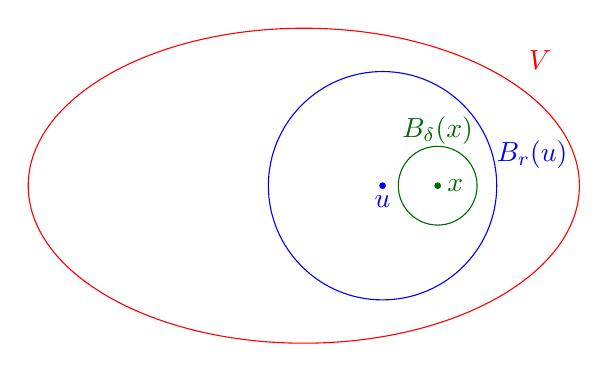
\begin{tikzpicture}
			\draw[red] (0,0) circle [x radius=3.5cm, y radius=2cm] ;
			\draw (3,1.6) node[red]{$V$};
			\draw [blue] (1,0) circle (1.45cm) ;
			\filldraw[blue] (1,0) circle (1pt) node[anchor=north]{$u$};
			\draw (2.9,0.4) node[blue]{$B_r(u)$};
			\draw [green!40!black] (1.7,0) circle (0.5cm) node [yshift=0.7cm]{$B_{\delta}(x)$} ;
			\filldraw[green!40!black] (1.7,0) circle (1pt) node[anchor=west]{$x$};
		\end{tikzpicture}
	\end{center}

	Given $x\in B_r(u)\subset V$, we want $\delta>0$ such that $x\in B_{\delta} (x)\subset B_r(u)\subset V$. Let $d=d(u,x)$. Choose $\delta $ such that $d+\delta<r$ (e.g. $\delta<\frac{r-d}{2}$)

	If $y\in B_{\delta}(x)$ we will be done by showing that $d(u,y)<r$ but $$d(u,y)\leq d(u,x)+d(x,y)<d+\delta<r$$
\end{myproof}

\cor{}{By the result of the proof, we can then show...}
\mlenma{}{Suppose $\vec{v_1}, \dots, \vec{v_n} \in \RR[n]$ is subspace of $\RR^n$.}
\mprop{}{$1 + 1 = 2$.}

\section{Random}
\dfn{Normed Linear Space and Norm $\boldsymbol{\|\cdot\|}$}{Let $V$ be a vector space over $\bbR$ (or $\bbC$). A norm on $V$ is function $\|\cdot\|\ V\to \bbR_{\geq 0}$ satisfying \begin{enumerate}[label=\bfseries\tiny\protect\circled{\small\arabic*}]
		\item \label{n:1}$\|x\|=0 \iff x=0$ $\forall$ $x\in V$
		\item \label{n:2}	$\|\lambda x\|=|\lambda|\|x\|$ $\forall$ $\lambda\in\bbR$(or $\bbC$), $x\in V$
		\item \label{n:3} $\|x+y\| \leq \|x\|+\|y\|$ $\forall$ $x,y\in V$ (Triangle Inequality/Subadditivity)
	\end{enumerate}And $V$ is called a normed linear space.

	$\bullet $ Same definition works with $V$ a vector space over $\bbC$ (again $\|\cdot\|\to\bbR_{\geq 0}$) where \ref{n:2} becomes $\|\lambda x\|=|\lambda|\|x\|$ $\forall$ $\lambda\in\bbC$, $x\in V$, where for $\lambda=a+ib$, $|\lambda|=\sqrt{a^2+b^2}$ }


\ex{$\bs{p-}$Norm}{\label{pnorm}$V={\bbR}^m$, $p\in\bbR_{\geq 0}$. Define for $x=(x_1,x_2,\cdots,x_m)\in\bbR^m$ $$\|x\|_p=\Big(|x_1|^p+|x_2|^p+\cdots+|x_m|^p\Big)^{\frac1p}$$(In school $p=2$)}
\textbf{Special Case $\bs{p=1}$}: $\|x\|_1=|x_1|+|x_2|+\cdots+|x_m|$ is clearly a norm by usual triangle inequality. \par
\textbf{Special Case $\bs{p\to\infty\ (\bbR^m$ with $\|\cdot\|_{\infty})}$}: $\|x\|_{\infty}=\max\{|x_1|,|x_2|,\cdots,|x_m|\}$\\
For $m=1$ these $p-$norms are nothing but $|x|$.
Now exercise
\qs{}{\label{exs1}Prove that triangle inequality is true if $p\geq 1$ for $p-$norms. (What goes wrong for $p<1$ ?)}
\sol{\textbf{For Property \ref{n:3} for norm-2}	\subsubsection*{\textbf{When field is $\bbR:$}} We have to show\begin{align*}
		         & \sum_i(x_i+y_i)^2\leq \left(\sqrt{\sum_ix_i^2} +\sqrt{\sum_iy_i^2}\right)^2                                       \\
		\implies & \sum_i (x_i^2+2x_iy_i+y_i^2)\leq \sum_ix_i^2+2\sqrt{\left[\sum_ix_i^2\right]\left[\sum_iy_i^2\right]}+\sum_iy_i^2 \\
		\implies & \left[\sum_ix_iy_i\right]^2\leq \left[\sum_ix_i^2\right]\left[\sum_iy_i^2\right]
	\end{align*}So in other words prove $\langle x,y\rangle^2 \leq \langle x,x\rangle\langle y,y\rangle$ where
	$$\langle x,y\rangle =\sum\limits_i x_iy_i$$

	\begin{note}
		\begin{itemize}
			\item $\|x\|^2=\langle x,x\rangle$
			\item $\langle x,y\rangle=\langle y,x\rangle$
			\item $\langle \cdot,\cdot\rangle$ is $\bbR-$linear in each slot i.e. \begin{align*}
				      \langle rx+x',y\rangle=r\langle x,y\rangle+\langle x',y\rangle	\text{ and similarly for second slot}
			      \end{align*}Here in $\langle x,y\rangle$ $x$ is in first slot and $y$ is in second slot.
		\end{itemize}
	\end{note}Now the statement is just the Cauchy-Schwartz Inequality. For proof $$\langle x,y\rangle^2\leq \langle x,x\rangle\langle y,y\rangle $$ expand everything of $\langle x-\lambda y,x-\lambda y\rangle$ which is going to give a quadratic equation in variable $\lambda $ \begin{align*}
		\langle x-\lambda y,x-\lambda y\rangle & =\langle x,x-\lambda y\rangle-\lambda\langle y,x-\lambda y\rangle                                       \\
		                                       & =\langle x ,x\rangle -\lambda\langle x,y\rangle -\lambda\langle y,x\rangle +\lambda^2\langle y,y\rangle \\
		                                       & =\langle x,x\rangle -2\lambda\langle x,y\rangle+\lambda^2\langle y,y\rangle
	\end{align*}Now unless $x=\lambda y$ we have $\langle x-\lambda y,x-\lambda y\rangle>0$ Hence the quadratic equation has no root therefore the discriminant is greater than zero.

	\subsubsection*{\textbf{When field is $\bbC:$}}Modify the definition by $$\langle x,y\rangle=\sum_i\overline{x_i}y_i$$Then we still have $\langle x,x\rangle\geq 0$}

\section{Algorithms}
\begin{algorithm}[H]
\KwIn{This is some input}
\KwOut{This is some output}
\SetAlgoLined
\SetNoFillComment
\tcc{This is a comment}
\vspace{3mm}
some code here\;
$x \leftarrow 0$\;
$y \leftarrow 0$\;
\uIf{$ x > 5$} {
    x is greater than 5 \tcp*{This is also a comment}
}
\Else {
    x is less than or equal to 5\;
}
\ForEach{y in 0..5} {
    $y \leftarrow y + 1$\;
}
\For{$y$ in $0..5$} {
    $y \leftarrow y - 1$\;
}
\While{$x > 5$} {
    $x \leftarrow x - 1$\;
}
\Return Return something here\;
\caption{what}
\end{algorithm}
\fi
\end{document}